% This is the Reed College LaTeX thesis template. Most of the work
% for the document class was done by Sam Noble (SN), as well as this
% template. Later comments etc. by Ben Salzberg (BTS). Additional
% restructuring and APA support by Jess Youngberg (JY).
% Your comments and suggestions are more than welcome; please email
% them to cus@reed.edu
%
% See http://web.reed.edu/cis/help/latex.html for help. There are a
% great bunch of help pages there, with notes on
% getting started, bibtex, etc. Go there and read it if you're not
% already familiar with LaTeX.
%
% Any line that starts with a percent symbol is a comment.
% They won't show up in the document, and are useful for notes
% to yourself and explaining commands.
% Commenting also removes a line from the document;
% very handy for troubleshooting problems. -BTS

% As far as I know, this follows the requirements laid out in
% the 2002-2003 Senior Handbook. Ask a librarian to check the
% document before binding. -SN

%%
%% Preamble
%%
% \documentclass{<something>} must begin each LaTeX document
\documentclass[12pt,twoside]{reedthesis}
% Packages are extensions to the basic LaTeX functions. Whatever you
% want to typeset, there is probably a package out there for it.
% Chemistry (chemtex), screenplays, you name it.
% Check out CTAN to see: http://www.ctan.org/
%%
\usepackage{graphicx,latexsym}
\usepackage{amsmath}
\usepackage{amssymb,amsthm}
\usepackage{longtable,booktabs,setspace}
\usepackage{chemarr} %% Useful for one reaction arrow, useless if you're not a chem major
\usepackage[hyphens]{url}
% Added by CII
\usepackage{hyperref}
\usepackage{lmodern}
\usepackage{float}
\floatplacement{figure}{H}
% End of CII addition
\usepackage{rotating}

% Next line commented out by CII
%%% \usepackage{natbib}
% Comment out the natbib line above and uncomment the following two lines to use the new
% biblatex-chicago style, for Chicago A. Also make some changes at the end where the
% bibliography is included.
%\usepackage{biblatex-chicago}
%\bibliography{thesis}


% Added by CII (Thanks, Hadley!)
% Use ref for internal links
\renewcommand{\hyperref}[2][???]{\autoref{#1}}
\def\chapterautorefname{Chapter}
\def\sectionautorefname{Section}
\def\subsectionautorefname{Subsection}
% End of CII addition

% Added by CII
\usepackage{caption}
\captionsetup{width=5in}
% End of CII addition

% \usepackage{times} % other fonts are available like times, bookman, charter, palatino

% Syntax highlighting #22

% To pass between YAML and LaTeX the dollar signs are added by CII
\title{Forecasting Constituents of the MSCI Minimum Volatility Index Through
Logistic Regression}
\author{John A. Gilheany}
% The month and year that you submit your FINAL draft TO THE LIBRARY (May or December)
\date{November 6, 2017}
\division{The Faculty of Arts and Sciences}
\advisor{Professor Michael Parzen}
\institution{Harvard University
\begin{figure}
\centerline{\includegraphics[height=1.5in]{/Users/johngilheany/Desktop/harvardlogo.jpg}}
\end{figure}}
\degree{Bachelor of Arts in Statistics (Honors)}
%If you have two advisors for some reason, you can use the following
% Uncommented out by CII
\altadvisor{David Kane}
% End of CII addition

%%% Remember to use the correct department!
\department{Statistics}
% if you're writing a thesis in an interdisciplinary major,
% uncomment the line below and change the text as appropriate.
% check the Senior Handbook if unsure.
%\thedivisionof{The Established Interdisciplinary Committee for}
% if you want the approval page to say "Approved for the Committee",
% uncomment the next line
%\approvedforthe{Committee}

% Added by CII
%%% Copied from knitr
%% maxwidth is the original width if it's less than linewidth
%% otherwise use linewidth (to make sure the graphics do not exceed the margin)
\makeatletter
\def\maxwidth{ %
  \ifdim\Gin@nat@width>\linewidth
    \linewidth
  \else
    \Gin@nat@width
  \fi
}
\makeatother

\renewcommand{\contentsname}{Table of Contents}
% End of CII addition

\setlength{\parskip}{0pt}

% Added by CII

\providecommand{\tightlist}{%
  \setlength{\itemsep}{0pt}\setlength{\parskip}{0pt}}

\Acknowledgements{
I would like to thank my thesis co-advisors, Professor Michael Parzen
and David Kane, for all of their mentorship and guidance throughout the
process. David helped spark my interest in the field of quantitative
finance while advising me, alongside Professor Parzen, for a statistics
research and reading class. Much of the literature I read then served as
the foundation for this thesis. David also supervised me directly while
I interned at Hutchin Hill Capital during January break, meeting with me
daily to discuss progress on my research. I am also very grateful to
David for meeting with me throughout the semester to give suggestions
and comments on my work. I cannot thank David enough for his time and
guidance. Professor Parzen has also been extremely helpful throughout
the writing process, offering countless revisions and edit suggestions.
I am grateful for Professor Parzen's statistical perspective, and
helping throughout the data collection and analysis portions. I would
also like to thank Professor Mark Glickman for reviewing my logistic
regression model and offering suggestions for improvement, and to my
friends and family for proofreading my thesis.
}

\Dedication{

}

\Preface{

}

\Abstract{
The low-risk anomaly is the term in academic literature for the
empirical regularity that low-volatility stocks perform as well or
better than high-volatility stocks (Baker, Bradley, \& Wurgler, 2011).
The MSCI Minimum Volatility Index is designed to exploit this effect by
holding a minimum variance portfolio of stocks. USMV is an
exchange-traded fund that tracks the index. I used information from
Wharton Research Data Services to calculate the trailing beta, trailing
volatility, and price to book ratio for each stock. Using this data, I
created a logistic regression model to calculate the probability of an
individual stock being a member of the index at the next rebalance. It
was found that stocks with lower beta and lower volatility are more
likely to be in the index in the next period.
}

% End of CII addition
%%
%% End Preamble
%%
%

\usepackage{amsthm}
\newtheorem{theorem}{Theorem}[chapter]
\newtheorem{lemma}{Lemma}[chapter]
\theoremstyle{definition}
\newtheorem{definition}{Definition}[chapter]
\newtheorem{corollary}{Corollary}[chapter]
\newtheorem{proposition}{Proposition}[chapter]
\theoremstyle{definition}
\newtheorem{example}{Example}[chapter]
\theoremstyle{definition}
\newtheorem{exercise}{Exercise}[chapter]
\theoremstyle{remark}
\newtheorem*{remark}{Remark}
\newtheorem*{solution}{Solution}
\begin{document}

% Everything below added by CII
  \maketitle

\frontmatter % this stuff will be roman-numbered
\pagestyle{empty} % this removes page numbers from the frontmatter
  \begin{acknowledgements}
    I would like to thank my thesis co-advisors, Professor Michael Parzen
    and David Kane, for all of their mentorship and guidance throughout the
    process. David helped spark my interest in the field of quantitative
    finance while advising me, alongside Professor Parzen, for a statistics
    research and reading class. Much of the literature I read then served as
    the foundation for this thesis. David also supervised me directly while
    I interned at Hutchin Hill Capital during January break, meeting with me
    daily to discuss progress on my research. I am also very grateful to
    David for meeting with me throughout the semester to give suggestions
    and comments on my work. I cannot thank David enough for his time and
    guidance. Professor Parzen has also been extremely helpful throughout
    the writing process, offering countless revisions and edit suggestions.
    I am grateful for Professor Parzen's statistical perspective, and
    helping throughout the data collection and analysis portions. I would
    also like to thank Professor Mark Glickman for reviewing my logistic
    regression model and offering suggestions for improvement, and to my
    friends and family for proofreading my thesis.
  \end{acknowledgements}

  \hypersetup{linkcolor=black}
  \setcounter{tocdepth}{2}
  \tableofcontents

  \listoftables

  \listoffigures
  \begin{abstract}
    The low-risk anomaly is the term in academic literature for the
    empirical regularity that low-volatility stocks perform as well or
    better than high-volatility stocks (Baker, Bradley, \& Wurgler, 2011).
    The MSCI Minimum Volatility Index is designed to exploit this effect by
    holding a minimum variance portfolio of stocks. USMV is an
    exchange-traded fund that tracks the index. I used information from
    Wharton Research Data Services to calculate the trailing beta, trailing
    volatility, and price to book ratio for each stock. Using this data, I
    created a logistic regression model to calculate the probability of an
    individual stock being a member of the index at the next rebalance. It
    was found that stocks with lower beta and lower volatility are more
    likely to be in the index in the next period.
  \end{abstract}

\mainmatter % here the regular arabic numbering starts
\pagestyle{fancyplain} % turns page numbering back on

\chapter{Introduction}\label{introduction}

The iShares Edge MSCI USA Minimum Volatility (USMV) Exchange Traded Fund
(ETF) is designed to track the investment results of the MSCI Minimum
Volatility USA index, which is composed of stocks with a lower
volatility than the general market. This can provide investors with
exposure to a portfolio with low risk that has historically declined
less in value than the broader market during economic downturns. The ETF
is comprised of 189 holdings, and is rebalanced two times per year, with
the intention of mirroring the changes made by the index. The purpose of
this dissertation is to create a logistic regression model that will
forecast which stocks will be added or removed from this ETF when it is
rebalanced, and to understand what factors are significant. The model
will take into account volatility attributes of each stock, as well as
others potentially significant predictor variables from prior studies.

\section{Low-Risk Anomaly}\label{low-risk-anomaly}

Several studies have shown that portfolios of low-risk stocks have
higher risk-adjusted returns than portfolios of high-risk stocks (Baker
et al., 2011). Low-risk stocks can be considered stocks with a low-beta
and/or low-volatility. This anomaly exists for several reasons including
the need for money managers to be compared to a benchmark and an
increased focus on relative rather than absolute risk. The MSCI Minimum
Volatility index helps investors take advantage of this anomaly.

\section{MSCI Minimum Volatility
Index}\label{msci-minimum-volatility-index}

The MSCI Minimum Volatility USA index constituents come from the MSCI
USA Index, which is roughly comprised of the top 600 US stocks by market
cap. This minimum volatility index is intended to have a lower beta,
lower volatility, lower cap bias, and contain more stocks with less risk
than its parent index, which contains US mid-cap and large-cap stocks.
On the last trading days of May and November, the index is rebalanced
twice a year. The index typically has around 180 constituents, with an
average of 20 new additions and 14 deletions every 6 months. Over the
last five years, the number of additions has ranged from 12 to 25, while
the deletions have been between 10 and 19. Changes to the index are
usually announced nine trading days before they are set to take place
(BlackRock, 2017).

Using the Barra Open Optimizer, the Minimum Volatility Index creates a
minimum variance portfolio of low-risk stocks as a subset from its
parent index of US large-cap and mid-cap stock. Using an estimated
security covariance matrix, the MSCI Minimum Volatility Index is the
product of the lowest absolute volatility, considering the constraints
(MSCI, 2013). Moreover, these additions are simply a relabeling of
existing stocks in the parent index and do not include new additions to
the parent index. The low-risk stocks chosen to be in the index are
determined by a set of constraints, like maintaining a certain sector or
country weight, relative to the parent index.

There are many specific constraints to the MSCI Minimum Volatility
Index. One is that an individual stock cannot exceed 1.5\%, or twenty
times the weight of the stock in the parent index. The minimum weight of
a security in the minimum volatility index is also capped at 0.05\%. The
index aims to keep the weight of specific countries within a 5\% range
of the weight in the parent index, or three times the weight of the
country in the parent index. Sector weights cannot deviate more than 5\%
from the sector weights in the parent index. One-way turnover of the
index is also maxed at 10\%. Thus, taking into account these
constraints, the Barra Open Optimizer creates the lowest absolute
volatility portfolio possible (Wynne, 2016).

\section{iShares MSCI Min Vol USA
ETF}\label{ishares-msci-min-vol-usa-etf}

An Exchange Traded Fund (ETF) is a collection of stocks and/or bonds in
a single portfolio that is traded on a major exchange (Hayes, 2017). As
a result, the price of an ETF fluctuates on a regular basis. Exchange
Traded Funds generally have more liquidity and lower fees when compared
to other alternative instruments like mutual funds. Owning an ETF can
allow investors to minimize risk, since owning an ETF is comparable to
owning a portfolio of many different stocks. This diversification comes
at lower costs and less effort for investors as well. ETFs can also
track an index, commodity, bond, or basket of all of the above.

The iShares Edge MSCI Min Vol USA ETF (USMV) is a Blackrock-managed ETF
that tracks the investment results of the MSCI Minimum Volatility USA
index. Unlike an ETF, which is publicly traded, an index is not. The
goal of the iShares MSCI Min Vol USA ETF (USMV) is to track the MSCI
Minimum Volatility USA index, but this is more complicated than it
seems. In addition to tracking stocks in this index, the ETF aims to
mirror returns of the index. Any difference between the ETF return and
actual index return is called tracking error. The tracking error is
often very small and can typically be around a tenth of a percent. This
error can come from indices being market capitalization weighted,
meaning that price fluctuations of each stock lead to the weighting
being changed by a ratio of its market cap against the market cap of all
stocks in the index (Fontinelle, 2009). With these stock weightings in
the index constantly changing and people buying in and out of ETFs
constantly, it is hard to track performance completely accurately.
However, ETFs very closely follow indices, as their tracking errors are
generally quite small. Thus, although ETF data is not the same as index
data, the two are extremely comparable.

\section{Regression Model}\label{regression-model}

A logistic regression model will be created, which can be transformed to
calculate a probability of a stock being a member of the Minimum
Volatility Index. A logistic regression model will be used since the
dependent variable is dichotomous. The predictor variables will include
52-week trailing volatility, 52-week trailing beta, price/book ratio,
and whether or not the stock was in the index 6 months before, during
the previous rebalancing. These attributes were chosen after looking at
the historical literature and understanding of the minimum volatility
index.

\section{Significance}\label{significance}

As mentioned, the purpose of this thesis is to create a logistic
regression model to that will calculate the probability of a stock being
in the Minimum Volatility Index. An accurate model will allow for a
better understanding of a stock's volatility attributes, and can lead to
an investment opportunity. There is substantial price movement whenever
a stock is added or removed from a large ETF, like USMV. When a stock is
added to the index, USMV will buy large amounts of that stock,
increasing the demand, and consequently, the market price for that
stock. If the stock is bought in advance of this large purchase, then an
investor can enjoy quick price appreciation of the stock. Moreover, if a
stock is removed from the Minimum Volatility Index, the ETF will sell
all current holdings of the stock, which will increase the supply of the
stock, driving down market price of the stock. If one were to short this
stock before that happened, he/she can also profit from that event.

A phenomena known as ETF front-running occurs when traders buy or sell
stocks in advance of ETF managers after they announce an exit or
entrance of a position (MacDonald, 2009). There is typically a slight
lag between an announcement of an ETF to add or remove a position and
the actual purchase or sale of the stock. By acting quickly, traders can
scalp profit by buying a stock before an ETF does, and selling it to
them later at a slight profit, or short-selling a stock before an ETF
exits the position, and then buying it back at the lower price. A model
that can accurately calculate the probability of a stock being in the
Minimum Volatility Index could be used to predict a stock's addition or
deletion from the index before rebalancing. This can allow traders to
similarly front-run USMV, but before the market is able to react,
leading to larger profit opportunities.

\chapter{Literature Review}\label{literature-review}

\section{Measures of Risk}\label{measures-of-risk}

Assuming an efficient market, one of the most widely accepted tenets of
investing is that one will be receiving higher reward for taking on more
risk. Presumably, if this were not true, nobody would partake in higher
risk investments. Some risks to consider when making an investment
include those with respect to the market, liquidity, credit, inflation,
and FX (Ontario, 2017). When quantifying risk for a company, one can
look at the standard deviation of the stock price. By looking at the
historical dispersion of data from the mean, or normal returns, one
finds the stock's volatility. These calculations are based only on the
price fluctuations of the stock and no other external factors
(Investopedia, 2015). Volatility is also one of the best indicators of
bankruptcy. The other common form of risk measurement in finance is
beta, which measures the stock's price volatility compared to that of
the stock market. The market is typically a benchmarked index relevant
to the stock; for a large-cap US stock, the associated index could be
the S\&P 500. Beta is calculated by taking the covariance of the stock
returns and the market returns, then dividing by the variance of the
market. Shown below is the formula for beta, where \(R_s\) represents
the return of the stock and \(R_m\) represents the return of the market:
\begin{figure}
$$ \beta = \frac{Cov(R_s, R_m)} {Var(R_m)}$$
\caption{Beta}
\end{figure}
This yields a coefficient, which can be interpreted: a beta value of 1
indicates the stock price and market move together identically, a beta
value of less than 1 indicates the stock is less volatile than the
market, and a beta value of greater than 1 indicates the stock is more
volatile than the market. Beta values can be negative as well, and hold
the same interpretation as positive beta values, with the difference
being that the stock price and market move in opposite directions. For
example, a beta of -1 would mean the stock and market have the same
volatility and changes in price, but that the performance is inversely
related. Thus, the first sentence of this paragraph can have many
meanings, but can be interpreted as saying that stocks with higher beta
or volatility will have higher expected return.

\section{Overview of the Low-Risk
Anomaly}\label{overview-of-the-low-risk-anomaly}

The low-risk Anomaly stems from the observation that portfolios of
low-risk stocks have higher risk-adjusted returns than portfolios of
high-risk stocks. This idea challenges a widely regarded financial
principle that investing in higher-risk stocks will generally result in
higher expected return. In several studies, portfolios of high-risk
stocks and low-risk stocks were constructed and rebalanced regularly to
reflect these characteristics, and the low-risk portfolios outperformed
the high-risk portfolios by a factor of several times, over long-periods
of time including 1929-2015 (Vliet \& Koning, 2016) and 1968-2008 (Baker
et al., 2011).

One of the explanations is the need for money managers to be compared to
a benchmark, such as an index like the S\&P 500. This is reasonable, as
many fund managers are charging fees to manage money, and need a way to
prove themselves and their abilities. By outperforming an index, a fund
manager is able to generate alpha, and presumably raise money money or
change higher fees. By underperforming an index, the fund managers have
a hard time justifying fee charges to clients, since they could just
invest in the index passively for little to no fee. Thus, much of the
risk for them is relative, coming from potentially underperforming on a
benchmark. Moreover, with this doubling of assets under active
management from 30\% to 60\% in 1968-2008, the low-risk anomaly
intensified. Another metric of fund manager performance is through the
``information ratio'' (IR), or the expected return difference between
the manager and the expected return of the S\&P 500, divided by the
volatility of this return difference (Goodwin, 1998). Shown below is the
formula for IR, where \(R_p\) represents the return of the portfolio,
\(R_i\) represents the return of the index, and \(\sigma_p\) represents
the standard deviation of portfolio returns:
\begin{figure}
$$ IR = \frac{(R_p - R_i)} {\sigma_p}$$
\caption{Information Ratio}
\end{figure}
The goal of an investment manager is to maximize this number, best as
possible, through picking stocks that will outperform the market. These
help to create a greater demand for higher-risk stocks while
discouraging investments in low-beta, low-volatility stocks, and
ultimately increases the market's appetite for risky stocks with high
reward potential, driving up price and driving down expected return.

In addition to the focus on relative rather than absolute risk, money
managers also often focus on single period returns, often as short as a
month, which aim to remove the effects of compounding. This helps
differentiate each manager's stock picking abilities, but ignores the
real-world and significance of compounding. Humans also have a
predisposition for the lottery effect, which is increased interest in
stocks with high skew - that is high upside potential. Risk can also be
decomposed into macro and micro-effects - that is, looking for and
comparing the risk-return characteristics of stocks with different risk
profiles, but similar country and industry risks. It turned out that the
micro-effects, those that were stock-specific, were statistically
significant at generating alpha, while the macro-effects, those that
were country and industry-specific was not. These literature reviews
also examine both volatility and beta as a measure of risk and suggest
that beta is not an adequate risk metric. In fact, though beta and
volatility are obviously very correlated, beta appears to be more
related to this low-risk anomaly than volatility. This can have
significant implications on the significance of the predictor variables
in the logistic regression model in this dissertation.

There are many real-world trading strategies that utilize this anomaly.
One example includes betting against Beta (BaB), which is a strategy
used by quantitative hedge funds like AQR. Betting against Correlation
(BaC) is a similar strategy in that it decomposes the effects of beta
into two separate factors for a more concentrated investment. Moreover,
index additions and deletions have proven to be instrumental in
influencing the price of affected stocks, indicating that if a model can
predict these movements accurately beforehand, there is an additional
considerable arbitrage opportunity.

\section{Evidence of the Low-Risk
Anomaly}\label{evidence-of-the-low-risk-anomaly}

\subsection{1929-2015}\label{section}

Jan de Koning and Pim Van Vliet set out to investigate the question:
\emph{Do high-volatility stocks return more than low-volatility stocks?}
by constructing high-volatility and low-volatility portfolios, and
comparing the two over a 86-year time span, from 1929-2015. Over this
period, low-volatility stocks outperformed high-volatility stocks by a
factor of 18, excluding inflation and transaction costs. If both
portfolios started off with \$100 in 1929, the low-volatility portfolio
end value would be worth \$395,000, while the high-volatility portfolio
would be worth just \$21,000. In reality, these values would both be
much smaller if the costs of trading the stocks and inflation were
considered, but excluding them is reasonable as the effect on both
portfolios would be pretty similar. The low-volatility portfolio
returned 10.2\% annually whereas the high-volatility portfolio returned
just 6.4\% annually. This annual difference of 3.8\% is striking, and
when considering compounding over an 86-year period, helps explain why
the low-volatility portfolio's value was over 18 times that of the
high-volatility portfolio. In this study, the annualized volatility of
the low-volatility portfolio was 13\%, and the annualized volatility of
the high-volatility portfolio was around 2.5 times that, at 36\% (Vliet
\& Koning, 2016).

\subsection{1968-2008}\label{section-1}

Baker et al. performed a study similar to that done by van Vliet and de
Koning, but used 41 years of CRSP data, ranging from January 1968 --
December 2008. It is important to note the ranges of dates used; the
Great Recession began in 2007 after the bursting of the subprime
mortgage bubble, leading to the collapse of several large, investment
banks, and the government bailout of many others. This caused market
indices, like the Dow, to drop from a high in 2007 of 14,164.43 to
8,776.39 by December 2008, representing a decrease in over 38\% during
that period (Amadeo, 2017). Thus, just as van Vliet and De Koning
started their sample right before the Great Depression to help amplify
their results, Baker, Bradley, and Wurgler ended their sample after the
Great Recession. Though this may help amplify the results, this does not
take away from the significance of the findings (Baker et al., 2011).

Baker et al. constructed low-volatility, high-volatility, low-beta, and
high-beta portfolios using the top 1,000 stocks by market capitalization
and then calculated each stock's five-year trailing volatility or beta.
A dollar investment in the low-volatility portfolio in 1968 appreciated
to \$59.55 by 2008, or \$10.12 in real terms, when accounting for
inflation. On the other hand, the highest-volatility portfolio went from
a dollar in value to just 58 cents from 1968-2008, with a real value of
around 10 cents, when considering inflation. Thus the low-volatility
portfolio outperformed the high-volatility portfolio by over 100 times
both in terms of nominal and real value. When using beta as a measure
for risk, the finding was very similar. In the lowest-beta portfolio, a
dollar grew to \$60.46 in nominal value throughout the 41-year period,
or \$10.28 in real value after considering inflation. The highest-beta
portfolio grew from a dollar to \$3.77 in nominal terms, or \$0.64 in
real terms after accounting for the effects of inflation. Thus, the
low-beta portfolio outperformed the high-beta portfolio by a factor of
16, in both nominal and real terms. One interesting observation here is
though both the low-beta and low-volatility portfolios outperformed the
high-beta and high-volatility portfolios, respectively, the discrepancy
was far more pronounced in the case of the the volatility portfolios.
Another significant observation was that investors who owned either the
high-beta or high-volatility portfolio in 1968 would have lost money
when accounting for the effects of inflation by 2008. It is also
important to note that this was just the case for large-cap companies,
as these portfolios were constructed from the top 1,000 stocks in terms
of market capitalization. The fact that this anomaly was observed for
large-cap companies is quite impressive, given there are generally a
lesser degree of mispricing in that realm than with small-cap companies,
because many small-cap stocks are not big enough for institutional
investors to invest in. Thus, this anomaly would be larger if the study
had been done for small-cap stocks instead. In addition, the portfolio
end values assumed no transaction costs, which in reality would have
been considered. The high-beta and high-volatility portfolios also cost
more to rebalance on a monthly level, as was done in the paper, than the
low-beta and low-volatility portfolios, indicating this anomaly is
actually more pronounced than initially reported. Baker et al. noted
that while high-beta portfolios outperformed the low-beta portfolios in
up-markets and underperformed the low-risk portfolios in down-markets,
that the low-beta anomaly persisted in both situations. On a
market-adjusted basis, low-beta consistently generates high alpha (Baker
et al., 2011). This was consistent with prior research (Pettengill,
Sundaram, \& Mathur, 1995).

\subsection{Critique of the Capital Asset Pricing
Model}\label{critique-of-the-capital-asset-pricing-model}

These findings are not new or revolutionary and have been observed in
many previous academic articles. Black, Jensen, and Scholes evaluated
some of the assumptions and effectiveness of the Capital Asset Pricing
Model (CAPM) (Jensen, Black, \& Scholes, 1972). CAPM is a model that
quantifies the relationship between risk and expected return for a
stock, and considers that investors should be compensated for the time
value of their money and risk they are taking. This is calculated as the
risk free rate plus the beta times the difference between the risk free
rate and expected market return (Brennan, 1989). Shown below is the
calculation for the expected return on an asset, \(\bar{r_a}\), where
\(r_f\) represents the risk-free rate, \(\beta\) represents the stock's
beta, and \(\bar{r_m}\) represents the expected market return:
\begin{figure}
$$ \bar{r_a} = r_f + \beta(\bar{r_m}-r_f)$$
\caption{Capital Asset Pricing Model}
\end{figure}
This will give the expected return of the stock, and anything in excess
of this will be considered alpha. Black, Jensen, and Scholes were able
to find that expected excess return, alpha, was not strictly
proportional to Beta, as it is mathematically in the CAPM. In 1975,
Haugen and Heins similarly found that there was little support for the
idea that risk premiums have manifested themselves in realized rates of
return. In fact, they pointed out that the relationship between risk and
return is much flatter than it is in the CAPM (Haugen \& Heins, 1975).
Twenty years later, Fama and French famously declared that beta was dead
after finding a flat relationship between beta and stock returns (Fama
\& French, 1992). Many additional papers and researchers have added
evidence for disproving the Capital Asset Pricing Model, and even
suggest that beta may not be the correct measure of risk, meaning that
the relationship between risk and return is not what many people believe
it to be (Mullins, 1982). However, other models relating risk and return
have had difficulty gaining acceptance and widespread usage in the
finance industry.

\section{Explanations for the Low-Risk
Anomaly}\label{explanations-for-the-low-risk-anomaly}

\subsection{Compounding}\label{compounding}

To fully grasp the low-risk anomaly, it is important to understand that
a higher volatile stock or portfolio will move in greater magnitude than
the underlying market. This holds true for both downside and upside
scenarios. When the market increases in value, a high-volatility stock
will increase in excess of this. For example, if the market increases by
20\% in one year, a high-volatility portfolio would reasonably
appreciate by more than 20\% over the same period. However, when the
market declines, a high-volatility portfolio would be expected to
decrease in excess of this amount. For instance, if the market decreases
by 20\% in one year, a high-volatility portfolio would reasonably
depreciate by more than 20\% over the same period. Lower-volatility
portfolios would react in similar fashion, just with a lesser magnitude
with respect to the market. With this in mind, one way the
low-volatility portfolio is able to outperform the higher-volatility
portfolio is by losing less during times of financial stress. Pim van
Vliet and Jan De Koning conveniently started their analysis right at the
beginning of the most severe economic depression in American history,
the Great Depression (Vliet \& Koning, 2016). The Great Depression began
in 1929 and eroded away around 80\% of the market's value by the time
the recovery began in 1932 (History, 2010). With this in mind, by 1932
the high-volatility portfolio declined by over 80\% while the
low-volatility portfolio declined by less than 80\%. More specifically,
the high-volatility portfolio shrunk from \$100 in value to just \$5
while the low-volatility portfolio shrunk from \$100 in value to \$30.
Thus, the results of this Vliet et al. could be taken with a grain of
salt, since although the portfolios each started off with the same
amount of money in 1929, the low-volatility portfolio was worth 6 times
as much as the high-volatility portfolio just four years later. However,
this is an expected consequence of the high-volatility portfolio, so
these results should not be discredited. With this being said, since the
low-volatility portfolio was able to lose less money during market
downturns, it is able to grow, or compound, its capital more effectively
than the high-volatility portfolio. To illustrate this, the portfolio
values can be considered in 1932, when the high-volatility portfolio
lost over 80\% in value. As Benjamin Graham, a famous value investor,
once noted the mathematical fact that ``once you lose 95\% of your
money, you have to gain 1,900\% just to get back where you started''
(Graham, 1965). Similarly, since the high-volatility portfolio lost six
times as much value as the low-volatility portfolio by 1932, it would
have to outperform the low-volatility portfolio by significantly more
than 600\% in order to return to the same value.

\subsection{Benchmarking}\label{benchmarking}

Thus, it seems very counterintuitive that fund managers and investors
would not only invest in low-volatility stocks, as it appears that these
stocks will outperform high-volatility stocks in the long-run. Part of
understanding why this is not a commonplace investment strategy for many
comes from interpreting what risk is defined as by the financial
community. To investors, risk is not necessarily analogous to
volatility, or even losing money. For many fund managers, risk comes
from underperforming a benchmark. David Blitz, the head of quantitative
equity research at Robeco, discussed the need for benchmarking the
performance of investment managers (Vliet \& Koning, 2016). Many
managers, especially of actively managed funds, command handsome
compensation in exchange for their investment acumen and diligence. Many
hedge funds have a ``Two and Twenty'' compensation structure, where the
managers charge a 2\% fee on total assets under management and take an
additional 20\% of profits (Investopedia, 2017). Given the large amount
of fees clients are paying, it is reasonable to believe that they expect
to receive a greater return than if they had invested in a passive,
market tracking ETF. These investment professionals need to prove to
their bosses and clients that they are above average at their job. For
example, if a hedge fund manager returns 10\% in one year, but the
market returns 10\% that same year, the client will be upset, as they
are now receiving a smaller return, given the hefty fees. In this case,
a \$100 investment in a market tracking index would return approximately
\$10 pre-tax, given there are little to no management fees. However,
\$100 invested in a hedge fund with a ``Two and Twenty'' structure would
yield the same initial \$10 pre-tax return, but the client would pay 2\%
of \$100 (\$2) in management fees, and 20\% of the \$10 profits (\$2) in
additional compensation. This would leave the client with a total of \$6
return, or 6\%, after all of the fees are paid out, and around half as
much as if they had invested in a market tracking ETF. As a result,
given the fee structure and client demands, active money managers are
often compared to a market benchmark like the S\&P 500; more
importantly, they are expected to outperform these benchmarks
substantially. Benchmarking also helps add perspective to a manager's
returns. If a manager returns 20\% in one year when the market returns
10\%, he/she will have many happy clients. However, if the manager
returns 20\% in the same year that the market returns 30\%, clients will
not be as pleased. This is a concept known as ``relative'' risk.

Some investors, like individuals saving for retirement, primarily care
about absolute risk, which is the total amount of money that is gained
or lost due to overall stock movements, with regard to the starting
amount of money invested. They will check their portfolio's total
performance without much concern for the exact market return. If their
portfolio gains 20\% in one year, they will be content, even if the
market increases 30\% in the same period. For these investors, the
horizon is long-term, so the short-term performance isn't as important
for them as it is for fund managers who may be trying to raise more
capital or justify high fees from clients. Volatility, in itself,
captures these changes in the price of a stock, and is an absolute risk
measurement. Many institutional investors do not look at risk on an
absolute level, as a retiree or mom-and-pop investor may, but instead
look at the risk of a portfolio with respect to the stock market or some
other widely accepted benchmark. For these investors, the risk is not so
much about losing money, rather it is more centered around lagging the
market or their peers. Investing is very much a relative game. To
further illustrate this idea, in relation to a fund manager, if a
portfolio drops 20\% while the market drops 40\%, this is seen as a much
better outcome than if a portfolio goes up 20\% while the market goes up
40\%. In the former, the manager lost money, but outperformed the market
by 20\%. In the latter, the manager made money but lagged the market by
20\%. This concept can be hard to fully grasp due to the natural bias
towards focus on absolute risk. Many have tried to explain this
seemingly misunderstood phenomena, including Jason Karceski, who noted
that an extrapolation bias could cause mutual fund managers to care more
about outperforming in a bull market, than underperforming in a bear
market (Karceski, 2002).

In fact, in 1968, institutional investors managed 30\% of all money, but
by 2008, the final year of the Baker et al. study, this figure increased
to 60\% (Baker et al., 2011). With this doubling of assets under active
management, the low-risk anomaly intensified. In addition to being
directly benchmarked against an index like the S\&P 500, fund managers
can also be compared using the ``information ratio'' (IR) which is the
expected return difference between the manager and the expected return
of the S\&P 500, divided by the volatility of this return difference
(tracking error) (Goodwin, 1998). The goal of an investment manager is
to maximize this number, as best possible, through picking stocks. In
fact, over 61\% of U.S. mutual fund managers are benchmarked against the
S\&P 500, while over 94\% are benchmarked to some U.S. index benchmark
(Sensoy, 2009). Moreover, SEC rules require mutual funds to compare
their performance to some benchmark (SEC, 2017). This intuitively makes
sense, as it allows investors to assess the skill and ability of
managers in an unbiased way, and also allows fund managers a chance to
differentiate themselves. However, this makes institutional investors,
who are managing the majority of the money in the United States, less
likely to buy low-volatility stocks, leading to higher prices and lower
expected returns for the high-volatility stocks and further exacerbating
the low-risk anomaly.

Going back to Baker's findings, it is very hard for fund managers to
attain a high IR with a low-risk portfolio. Part of this stems from the
need for investment managers without leverage to find mispriced stocks
with a beta very close to market risk (beta of 1), overweighting
positive-alpha stocks while underweighting negative-alpha stocks. When
comparing the Sharpe ratio of large cap stocks for a low-volatility
portfolio, it was found to be quite high at 0.38. However, the
Information Ratio was a very low 0.08, showing that this would be very
tough for a fund manager to have. To provide a comparison, during
1968-2008, the top value strategy portfolios had an IR of 0.51, and top
momentum strategy portfolios had an IR of 0.64. This is extremely high
compared to the IR of low-volatility stocks in this period, which ranged
from 0.08 to 0.17, showing these constructed low-beta portfolios would
be unlikely to be used by any fund manager. While beta and volatility
are undoubtedly very correlated, this shows that beta is more related to
the anomaly than volatility, especially with large cap stocks, which is
what most fund managers disproportionately focus their investments in
(Baker et al., 2011).

\subsection{Single-Period Returns}\label{single-period-returns}

Another explanation of the low-volatility anomaly is an increased focus
on returns over short-term periods by many researchers and investors. By
focusing on ``single period returns,'' which in most academic studies is
just a one-month period, the significance of compounding is removed.
This is more of an arithmetic way to calculate returns, where each
month's return can be averaged, for example. Mathematically, this is not
the correct way to calculate a return since it does remove the effect of
compounding, but is a common way to compare fund managers. Moreover,
when done over very short time periods (like a year), the effect of
compounding is not as significant as it is for very long-term periods.
To illustrate this, the following scenario can be considered: in one
month a portfolio worth \$100 drops 50\% to \$50, then the next month
increases 50\% to \$75. The investment return is dependent on how one
divides the time period. Looking at it on a monthly basis, even though
the portfolio lost \$25 in value, the net return would be -50\% +50\%,
or 0\% (with focus on single period returns, not accounting for
compounding). However, looking at it on a longer-term basis, the net
return was -25\%, as the \$100 portfolio ended up losing \$25 in value.
By not fully including the magic ``return upon return'' effect of
compounding, the high-volatility portfolio discussed earlier performed
more than 6\% better per year (Vliet \& Koning, 2016).

\subsubsection{Psychological and Behavioral
Factors}\label{psychological-and-behavioral-factors}

In addition to the reasons mentioned, there are several psychological
reasons why some investors are not attracted to low-risk stocks. Eric
Falkenstein, a renowned author in the low-volatility investing realm,
wrote that ``envy is at the root of the investment paradox''
(Falkenstein, 2012). Some investors simply don't recognize the
significance of compounding returns. Many others do but are unable to
utilize the paradox due to relative risk and career pressures. Analysts
who choose big winners are more likely to get recognized and promoted
than those who pick safer stocks with lower upside potential; funds that
pick the right high-risk stocks that turn out to be major home-runs will
see more reward as an increase in AUM, and consequently an uptick in
management fees. Moreover, some people do not invest in low-risk stocks
because they have less of an appeal than high-risk stocks, where
investors think they can make a lot of money easily and quickly. Even
the news will have a bias towards reporting about and covering stocks
that have become big winners. One famous big winner is Amazon: a \$5,000
investment in 1997 would be worth \$2,400,000 today, or an increase
49,000\% (Berger, 2017). With all the excitement and reporting to this
day on big winners like Amazon, many people forget about the number of
similar technology companies that failed during the dot-com bubble and
are worth nothing today. Thus, these high-risk stocks are more ``sexy''
and have a ``lottery ticket'' element that tempts investors with the
appeal of a big payday.

Many investors have a natural preference for lotteries, even though
there is a general aversion towards loss. If a stock has a positive
skew, which is defined as a larger probability of a large positive
payoff than probability of a small payoff, investors typically are very
interested (Baker et al., 2011). Though skew is not the same as
volatility, through their research, Boyer, Mitton, and Vorkink made a
strong case for how expected skewness is a proxy for volatility through
their findings that expected skewness assisted in explaining the
observation that stocks with high idiosyncratic volatility have low
expected returns (Boyer, Mitton, \& Vorkink, 2009).

Another idea is representativeness, or that Bayes' rule and probability
theory are often not natural to people, even in the most seasoned
investment professionals. One example of this is selectively looking at
a few speculative investments that have turned out to be massive
successes without considering the numerous failures. As mentioned
earlier, the news will focus on Amazon's great success over the past
twenty years, but will not focus as much on all of the tech stocks that
became worthless after the bubble burst. By not separating and
considering all winners and losers, the average investor may be inclined
to overpay for a riskier stock (Baker et al., 2011).

Overconfidence has also been tied to a preference for volatile stocks;
optimists are generally more aggressive than pessimists. In a study,
people were asked questions on how certain they were of their responses
and it appeared many did not have an understanding of probability.
Estimating the heat of a candle flame is very difficult, so for someone
to say they are 80\% sure of their answer is impressive, yet hard to
believe. This can apply when people are asked for a confidence interval
of the population of a city. In many instances, the person would be
confident and give a very narrow range of people (Fischhoff, Slovic, \&
Lichtenstein, 1977). This same concept applies when valuing stocks and
evaluating certain investment opportunities.

Overall, irrational investor preference for lotteries and
high-volatility stocks, as well as investment managers' focus on
benchmarks and IR, flatten and eventually invert the relationship
between risk and return in the long-run. Moreover, it has been shown by
Baker et al., and prior observations that the anomaly intensified with
the increase in assets under active management of fund managers in the
U.S. These reasons together have led to the findings that low-beta and
low-volatility stocks have outperformed high-beta, high-volatility
stocks from 1968-2008, in part due to combining great returns with low
downturns. Investor preference for ``lotteries'' and a bias of
overconfidence creates a higher demand for higher-volatility securities,
and the need to benchmark creates a greater demand for higher risk
stocks, while discouraging investments in low-beta, low-volatility
stocks. This understandably, increases the market's appetite for risky
stocks with high reward potential, driving up price and driving down
expected return. These reasons appear perennial, so the anomaly is
unlikely to cease to exist in the near future.

\subsection{Profitability}\label{profitability}

Defensive equity strategies generally aim at constructing a portfolio
comprised of more low-risk stocks. This strategy has been becoming very
popular as of late, in part due to equity markets that have suffered two
recent, severe downturns, negative nominal returns in the first decade
of 2000, and literature proving a weak or negative relationship between
risk and return (Novy-Marx, 2014). Prior literature has looked at the
relationship of performance relative to size and value, but many studies
have not done a deeper dive into the effect of specific factors, such as
profitability (Chan, Hamao, \& Lakonishok, 1991). In fact, it has been
shown that high profitability is the most significant predictor of
low-volatility, inherently causing these defensive equity strategies to
indirectly tilt towards profitability, in addition to the more known
factors, like size and value. Size is very important, as small growth
stocks are typically underweight in these strategies, while large value
stocks are overweight. Likewise, value stocks are typically overweight,
while growth stocks are underweight. Thus, the performance of defensive
equity strategies can be explained by accounting for size, value, and
profitability (Novy-Marx, 2014).

In terms of performance, defensive equity strategies, which are defined
as low-volatility or low-beta in nature, have outperformed more
aggressive strategies. This was already shown between 1929-2008 (Vliet
\& Koning, 2016) and in a separate study from 1968-2015 (Baker et al.,
2011), but Novy-Marx analyzes a different timeframe. He looks at the
characteristics of these low-risk portfolios in more detail by analyzing
log-likelihood ratios that a stock selected at random is of a given
style, like size or value, relative to the unconditional probability of
being that style (Novy-Marx, 2014). The findings were very telling: on
average, low-volatility stocks were 30 times larger than high-volatility
stocks. As a result, though the high-volatility names made up half the
total number of stocks, they contributed to just 9\% of the total market
capitalization when compared with low-volatility stocks. Moreover, when
looking at the average returns across the portfolios of various
volatilities, there seemed to be a relatively flat, slightly increased
return with increasing volatility. The high-volatility/high-beta
portfolio had a significant negative alpha, while the
low-volatility/low-beta portfolio had a significant positive alpha
(Novy-Marx, 2014).

Many of the volatile stocks tended to be small, unprofitable growth
stocks which can help explain the relationship of the defensive strategy
performance to size, value, and profitability. In fact, since 1968-2015,
the portfolio of high-volatility stocks almost mirrored the performance
of the portfolio of unprofitable, small growth stocks. Thus, the
outperformance of defensive stocks from 1968-2015 have delivered
significant alpha and can be explained when accounting for size, value,
and profitability. In fact, profitability itself is so significant, that
the case can be made that this alpha may come in large part from
excluding unprofitable, small growth stocks (Novy-Marx, 2014).

\section{Decomposition of the Low-Risk Anomaly into Micro and Macro
Effects}\label{decomposition-of-the-low-risk-anomaly-into-micro-and-macro-effects}

The low-beta anomaly can be further broken up into micro and macro
effects. The micro effects can be observed through picking low-beta
stocks, and keeping country and industry risk the same, while the macro
effects can be isolated by picking low-beta countries or industries,
while keeping stock-specific risk the same. Baker et al. generates
observable micro effects by creating portfolios of equity longs and
shorts, holding forecasted country and industry risk constant. The macro
effects were observed by constructing long-short portfolios of various
countries and industries, holding forecasted stock-specific risk
constant. Studying a number of stocks within 29 industries and 31
different developed countries, the macro and micro effects were observed
and, both together, were shown to play an important role in explaining
the low-risk anomaly (Baker, Bradley, \& Taliaferro, 2014).

Looking at 31 developed countries including Canada, France, Germany,
Japan, and Singapore, Baker et al. worked to decompose the low-risk
anomaly into country and stock specific effects. Similar to the industry
findings, country-beta was able to predict stock betas to a certain
extent, but not as well as historical stock betas were. Looking only at
country betas yielded around half the risk reduction and two-thirds the
risk-adjusted return improvement, as compared to stock betas. This study
implied that predicting risk of individual stocks is in itself very hard
when only given data on country or industry risk, but when given all the
data can have much more predictive power (Baker et al., 2014).

It was found that using industry beta to predict future stock betas was
possible, but not as effective as just using historical stock betas.
Industry beta information without stock information does improve
risk-adjusted returns, just not to the same extent as stock information
does. Baker et al. go into detail trying to isolate pure-industry
effects and pure-stock effects. Pure-industry effects are the average
differences between high and low-beta industries, while holding constant
stock risk. Pure-stock risk is the opposite of that, calculating the
average difference between high-beta and low-beta stocks, keeping
industry risk constant. In the end, finding low-risk portfolios using
selection of low-risk stocks and keeping industry constant was around
four times more effective than using low-risk industries and keeping
stock risk constant. However, once again, using the historical betas of
both together, has more predictive power than either one alone (Baker et
al., 2014).

Micro-selection of stocks, holding country and industry risks constant,
was shown to significantly reduce risk without a significant decrease in
return. In some cases, high-risk stocks within particular industries
were able to be distinctly identified, and they typically had similar
returns when compared to low-risk stocks in the same industry and
country. Macro-selection, which involved holding stock-specific risks
constant, was shown to lead to increases in return with small
differences in risk, especially with regards to the country chosen.
Stocks in high-risk countries were found to have distinctly lower
returns than low-risk countries. These findings hold significant
investment opportunity, due to the implication that people seeking
arbitrage opportunities through mispricing of macro-effects like
industry and sector, or through ETFs might not be as successful as
exploiting the risk reduction opportunities stemming from micro-effects.
While both the micro and macro-effects led to higher CAPM alpha by
reducing risk and increasing returns, only the micro-effects were found
to be statistically significant, whereas the macro-effects of country
selection and industry selection were not found to be statistically
significant. Thus, there is more of an arbitrage opportunity exploiting
the micro-effects of individual stock selection than the macro-effects
like country to industry. Even though the macro-effects have many
limitations in practice, micro-effects are also limited due to leverage
restrictions and benchmark mandates.

\section{Applications of the Low-Risk
Anomaly}\label{applications-of-the-low-risk-anomaly}

\subsection{Betting Against Beta (BaB)}\label{betting-against-beta-bab}

Prior studies suggest that beta is not a great measure of risk and is
more related to the anomaly than volatility is. AQR, a successful
quantitative-focused hedge fund, employs a strategy called Betting
Against Beta (BaB), which is a simple method of statistical arbitrage
generated by shorting high-beta stocks and longing low-beta stocks
(Investopedia, 2015). As discussed in some of the works previously, the
premise behind this arbitrage opportunity is that high-beta stocks are
overpriced while low-beta stocks are underpriced. The theory is that the
stocks will eventually return to this equilibrium point, called the
security market line (SML). While the prices approach this median, the
investor can capture this spread as an arbitrage opportunity
(Investopedia, 2015).

The Capital Asset Pricing Model calculates the expected equity return
given certain levels of risk. Any excess above this risk-adjusted return
is the Sharpe Ratio, or alpha that is generated by the stock. The Sharpe
Ratio is calculated by taking the mean portfolio return and subtracting
the risk free rate, then dividing by the standard deviation of portfolio
returns (Investopedia, 2017). Shown below is the formula for the Sharpe
Ratio, where \(\bar{r_p}\) represents the expected return of the
portfolio, \(r_f\) represents the risk-free rate, and \(\sigma_p\)
represents standard deviation of portfolio returns:
\begin{figure}
$$ SR = \frac{\bar{r_p}-r_f} {\sigma_p} $$
\caption{Sharpe Ratio}
\end{figure}
Investors try to maximize this number, and one way to do it is by
levering up, or using borrowed capital to invest. By paying a fixed
interest rate on the borrowed capital, assuming the return is more than
the interest rate, an investor can increase the return on their invested
equity. As one may imagine, this is more risky, as returns in both the
upward and downward direction are magnified. As a result, many
investment managers, like mutual funds, are legally constrained on the
amount of leverage they can apply to a portfolio. Due to this, many fund
managers must overweight high-beta stocks to improve overall returns.
This leads to a tilting towards beta, and a flattening of this SML in
relation to CAPM. This leads to a pricing anomaly which firms like AQR
can take advantage of. By creating a market neutral strategy, and
shorting high-beta stocks while longing low-beta stocks, they can
capture this opportunity.

Andrea Frazzini and Lasse Heje Pedersen of AQR describe this strategy
through a model in one of their studies (Frazzini \& Pedersen, 2014). In
this paper, a real-world resembling model is created with leverage and
margin constraints in 55,600 stocks from 20 global stock, bond, credit,
and future markets. Some agents in this model cannot use any leverage,
and some have limited margin constraints, much like many investors and
fund managers. As mentioned, many mutual funds, pension funds, and
individual investors are constrained by the amount of leverage they can
take on, such that instead of investing in a portfolio yielding the
highest Sharpe Ratio, they are forced to overweight portfolios with
riskier stocks. This suggests fund managers hold high-beta stocks to a
lower risk adjusted return standard than low-beta stocks, which would
require leverage. Thus, if someone cannot leverage or has significant
leverage constraints, then they will overweight riskier securities. The
model in this paper was able to empirically show this in the equities,
bonds, and futures markets. This was done by sorting portfolios by
betas, and realizing alphas and Sharpe Ratios declined with increases in
portfolio-beta (Frazzini \& Pedersen, 2014).

Presumably, if one could lever up without constraint, the investor would
underweight high-beta assets and overweight low-beta assets. BaB factors
help explain this. A BaB factor is a portfolio longing low-beta
securities (leveraged to a beta of 1), shorting high-beta assets
(deleveraged to a beta of 1), that is market neutral. Frazzini's model
predicts that this portfolio will have a positive return that increases
with the spread in the betas and tightness of leverage constraints.
Thus, being long low-beta stocks and short high-beta stocks yields
significant, and positive risk-adjusted returns. This was observed in
the model by looking at U.S., developing, and international equity
markets and noting that the BaB factor yielded a Sharpe ratio that was
double its value effect, and 40\% greater than momentum. The BaB factor
had very high risk-adjusted returns, and during four twenty-year periods
between 1926 and 2012, produced significant positive returns. This
generally held across other asset classes, too, including credit and
treasury bond markets (Frazzini \& Pedersen, 2014).

When a leverage constraint was met or surpassed, and the agent needs to
deleverage, the BaB factor portfolio experiences negative returns, but
its expected future returns still increased. This was once again shown
with a time series with spreads of various funding constraints. Another
central idea of the model was that increased funding liquidity risk
compresses betas toward one. Frazzini et al. proved this by looking at
the volatility of funding constraints as funding liquidity risk; the end
finding was that the dispersion of betas when funding liquidity risk is
high, and was much lower than when funding liquidity risk is low. In
other words, tightening of funding constraints leads to a lower BaB
factor (Frazzini \& Pedersen, 2014).

Finally, the model showed that investors who are more
leverage-constrained are forced to overweight riskier securities, while
investors without such constraints could overweight low-risk securities.
Observing a number of stock portfolios from constrained investors showed
most fund managers and individual investors' portfolios have a beta
greater than one. However, many private equity firms that perform
leveraged buyouts are traditionally able to purchase firms with a beta
below one and apply leverage, allowing them to utilize this anomaly due
to the the fact that they have lower leverage constraints than their
public market counterparts. Famed investor Warren Buffett even bets
against beta, as many of his investments are leveraged, low-beta stocks.
By having these constraints, though, the typical public markets investor
is forced to hold on to riskier, high-beta stocks, leading to
effectiveness of the BaB factor (Frazzini \& Pedersen, 2014).

\subsection{Betting Against Correlation
(BaC)}\label{betting-against-correlation-bac}

In trying to understand the low-risk anomaly and how it could be
applied, Asness et al. considered two possible explanations. The first
looked at whether it was caused by leverage constraints, or measurement
using systematic risk. The second focused on the behavioral effects, or
idiosyncratic risks. One of the main issues with prior research is that
many low-risk factors are correlated and interrelated, making it hard to
completely isolate certain factors or effects. Adrian et al. showed a
link between return of the BaB factor and financial intermediary
leverage (Adrian, Etula, \& Muir, 2014). Many of these factors,
including BaB, generally exhibited the ``low-risk effect'' and were
consequently very difficult to completely distinguish from one another.

Asness et al. attempted to clarify this by introducing a couple new
factors meant to control for existing factors (Asness, Frazzini,
Gormsen, \& Pedersen, 2016). They broke down BaB into two separate
factors: betting against correlation (BaC) and betting against
volatility (BAV). This was done because beta itself is calculated by
taking the stock's correlation with the market times its own volatility
and dividing by the market's overall volatility. BaC is accomplished
through longing stocks with a low correlation to the market, and
shorting those with a high correlation to the market, while trying to
match the volatilities of both the long and short portfolios. BAV is
achieved in a similar manner, except through longing stocks with
low-volatility and shorting high-volatility stocks while keeping
correlation constant.

To address the behavioral explanation, Asness et al. looked at some
prior factors from observations made by Ang et al. (Ang, Hodrick, Xing,
\& Zhang, 2006). They found that stocks with low idiosyncratic
volatility (IVOL) had a greater risk-adjusted return, and in 2009 added
to this by finding that a low maximum return (LMAX), a measure of
idiosyncratic skewness, is associated with greater risk-adjusted returns
(Ang, Hodrick, Xing, \& Zhang, 2009). Asness et al. kept the focus on
the LMAX and IVOL, but added another factor, scaled MAX (SMAX), which
longs stocks with a low MAX return divided by ex-ante volatility, and
consequently shorts stocks with a high MAX return divided by ex-ante
volatility (Asness et al., 2016). This allows focus on the lottery
demand, holding volatility relatively constant and only focusing on the
distribution of the returns. Margin debt held by investors and investor
sentiment were also noted.

Overall, 58,415 stocks from the MSCI World Index from 24 different
countries between January 1926 and December 2015 were covered (Asness et
al., 2016). BAV and BaC were found to be very successful in controlling
for the other factors that could influence the ``low-risk effect.'' The
BAV findings are in line with prior findings, and can be explained
through behavioral effects like the lottery preference and leverage
aversion. For all stocks, the BaC factor produced a significant
six-factor alpha that was nearly independent of the other low-risk
factors studied. This was partially due to the leverage aversion, which
indicates correlation changes in beta should be priced in. In terms of
explaining the behavioral side with factors, SMAX was the only truly
great, resilient measure used. The rest generally had higher turnover,
and were consequently very susceptible to microstructure noise. SMAX
attained positive risk-adjusted returns in the U.S. but negative
risk-adjusted returns globally, which was seen with some other
idiosyncratic risk factors. Asness et al. showed that systemic low-risk
factors generally tended to outperform behavioral risk factors,
especially when considering turnover and time period length. All in all,
the low-risk effect was believed to be driven by multiple factor
effects, meaning both leverage constraints and lottery demand could play
a role in influencing this. However, leverage constraint effects were a
bit stronger, especially internationally. By cleaning up these factors,
clearer explanations for previously observed results were provided
(Asness et al., 2016).

\subsection{Stock Price Response to Index
Rebalancing}\label{stock-price-response-to-index-rebalancing}

One of the driving fundamental assumptions of finance is a flat demand
curve for stocks, where risk is the main driver and each stock has a
perfect substitute. However, this concept has been questioned for the
past few years, with literature picking up on stocks showing supply
shocks and quantifying how this affects their market price. Literature
has shown several instances where large block sales of stock has
negatively affected its price (Harris \& Gurel, 1986). This was often
due to information contamination, which is new, significant information
about the company in the market. This information often reflects
fundamental changes in the company, and, if it is negative, will
understandably trigger block sales. Thus, the price change could be less
due to the supply shock, and caused more by fundamental changes in the
company's value, such as a scandal or earnings report release.

However, interesting patterns that have not yet been fully explained
emerge from observations regarding S\&P 500 company addition and
deletions. When companies are added or removed from the index, it is
often purely mechanical and usually not due to some drastic fundamental
change in the company. Assuming the market is efficient, the demand for
stocks should not change due to being added or removed from an index,
but several studies have shown that it does (Shleifer, 1986). The
studies agree that new additions to the S\&P come with higher than
normal returns for that company (Beneish \& Whaley, 1996). Though they
agree on the price movement, the studies tend to disagree on the precise
reason for this price movement; some possible explanations include:
compensation for providing liquidity, better monitoring for investors
when a company is added to a reputable and large index, and higher
analyst coverage leading to more information and analysis available on
the company (Chen, Noronha, \& Singal, 2004). One primary concern is
whether or not index reshuffling is an information-free event - that is,
whether a company being added or removed adds information about the
company to the market.

Others looked at factor index rebalancing for an information-free event
(Huij \& Kyosev, 2016). Factor indices are part of a parent index of
many other stocks and are constructed in a mechanical way that is
publicly available and usually based on ranking stocks off a particular
ratio of characteristic. The authors looked at one example, the MSCI
Minimum Volatility index, and recorded returns for the stocks that had
been added or dropped. It was found that the cumulative return from
announcement to the effective day was 1.07\% for stocks added with a
significant t-statistic of 7.16, with 62\% of the stocks exhibiting a
positive cumulative abnormal return. Of the 1.07\% increase, 0.63\% of
it was gained the following day, indicating that a large part of the
increase was due to greater demand from index funds. 0.31\% of the
return was lost five days after the rebalancing, but generally the price
tended to stabilize after around ten days. Thus, 68\% of the price
increase was long lasting while the other 32\% was temporary and lost
after a few days. This can be due to a liquidity premium charged by the
stock's owner or arbitrage activity. Average trading volume was also
significantly higher for stocks that were recently added to the index.
For the days between the announcement and actual addition of the stock,
the average trading volume was 30\% higher than normal, with a
significant t-statistic of 3.81. Moreover, there was a 74\% increase in
volume for the day prior to the actual addition of the security. A very
similar phenomena occurs with stocks set to be dropped from the USMV
Index; from the announcement of a stock being dropped to the day before
it is actually deleted from the index, the total cumulative abnormal
return was -0.91\%, and a total of -0.57\% came the day before. After
the stocks were deleted, 64\% had a negative return the following day,
and only 0.49\% of the -0.91\% was regained after three weeks. Trading
volume also spiked 46\% on the day prior to removal from the index.
After three weeks, it returned back to within 1\% of the normal trading
volume (Huij \& Kyosev, 2016).

These findings imply that once a security is added to a factor index,
the demand curve shifts to the right, moving the equilibrium. The
trading volume change is likely due to index funds buying or selling
massive amounts of the stocks that will be added or removed. Moreover,
it was found that the amount of the return is also directly related to
the weighting of the volume of stocks entering or leaving the factor
index. All in all, these findings suggest an index arbitrage opportunity
exists if index additions or deletions can be accurately predicted.

\chapter{Data Gathering Process}\label{data-gathering-process}

\section{Data Aggregation}\label{data-aggregation}

Data was collected for the iShares MSCI USA Equal Weighted ETF (EUSA),
which tracks the parent index of the minimum volatility index, and
iShares Edge MSCI Min Vol USA ETF (USMV), which tracks the minimum
volatility index, from Oct 31, 2011 to December 31, 2016 (BlackRock,
2017). The iShares data contained this information for the two ETFs of
interest for each constituent on the last trading day of every month.
This included characteristics of each stock, such as: ticker, company
name, asset class, weight of the stock relative to the entire index,
price per share, number of shares, market value of the position,
notional value of the position, sector, sedol number, isin number,
exchange that the stock is listed on, and the month end date for the
data. Each month-end dataset was individually downloaded, then
aggregated to create the two separate raw data sets - one for EUSA and
one for USMV. The data was then cleaned and stored in R (RStudio Team,
2015).

\section{Data Cleaning}\label{data-cleaning}

After having a quick overview of the data, there were many issues with
each respective dataset that needed to be fixed before the analysis
could occur. Since USMV is a subset of EUSA, the issues were very
similar, and those that existed in USMV, generally existed in USMV as
well. The issues could be broken down into 3 main types: erroneous
listed stock exchanges, problematic listed tickers, and price
discrepancies due to issues like stock splits. Moreover, cash and cash
related assets were removed from the data, as this dissertation focuses
only on the stocks.

\subsection{Non-US Exchanges}\label{non-us-exchanges}

Looking at the unique exchanges of the data, it was observed that there
were several foreign exchanges like the Swiss Exchange and the Mexican
Stock Exchange. Some of the stock exchanges from the data set are shown
below:
\begin{verbatim}
[1] New York Stock Exchange Inc.                      
[2] NASDAQ                                            
[3] Bolsa Mexicana De Valores (Mexican Stock Exchange)
[4] Nyse Euronext - Euronext Paris                    
[5] Boerse Berlin                                     
[6] Tokyo Stock Exchange                              
17 Levels: Boerse Berlin Boerse Duesseldorf ... Tokyo Stock Exchange
\end{verbatim}
This did not make sense, given the ETF constituents are supposed to be
US-focused, meaning they should be listed on US-based exchanges. Of the
non-US exchange errors, they can be further broken up into two
subgroups: companies that were incorrectly listed overseas and are
actually listed on US exchanges, and companies that also are actually
listed on US exchanges but instead had their overseas exchange tickers
listed.

\subsubsection{Mislabeled Exchanges}\label{mislabeled-exchanges}

The first type of error involved companies that are actually listed on
either the NYSE and NASDAQ, but were listed on a foreign exchange in the
data and still had their US ticker used. One example was BAC (Bank of
America) which is listed on the NYSE, but was listed on the Swiss Stock
Exchange in the dataset:
\begin{verbatim}
  ticker                 name weight price       exchange       date
1    BAC BANK OF AMERICA CORP 0.5812  6.83 Swiss Exchange 2011-10-31
2    BAC BANK OF AMERICA CORP 0.4643  5.44 Swiss Exchange 2011-11-30
3    BAC BANK OF AMERICA CORP 0.4732  5.56 Swiss Exchange 2011-12-30
4    BAC BANK OF AMERICA CORP 0.5823  7.13 Swiss Exchange 2012-01-31
5    BAC BANK OF AMERICA CORP 0.6235  7.97 Swiss Exchange 2012-02-29
6    BAC BANK OF AMERICA CORP 0.7375  9.57 Swiss Exchange 2012-03-30
\end{verbatim}
The price for BAC in the data set corresponded to the price of BAC in
the NYSE, even though it was listed on the Swiss Exchange; BAC also did
not corresponded to Bank of America on the Swiss Exchange. Thus, after
several checks, it could be concluded that BAC in the data set was
incorrectly listed on the Swiss Exchange, and should have been listed on
the NYSE instead. Since the ticker was still correct and would be read
in properly in the later stages of this paper, these cases were left as
is and no changes were made.

\subsubsection{Mislabeled Tickers}\label{mislabeled-tickers}

The second type of error stemmed from companies listed on foreign
exchanges that are also listed on a US exchange in reality, but had
their non-US ticker used in the data set. One example of this was Aflac,
Inc. which was listed by its ticker ``8686'' on the Tokyo stock
exchange:
\begin{verbatim}
  ticker       name weight price             exchange       date
1   8686 AFLAC INC. 0.1779 45.09 Tokyo Stock Exchange 2011-10-31
2   8686 AFLAC INC. 0.1719 43.44 Tokyo Stock Exchange 2011-11-30
3   8686 AFLAC INC. 0.1699 43.26 Tokyo Stock Exchange 2011-12-30
4   8686 AFLAC INC. 0.1810 48.23 Tokyo Stock Exchange 2012-01-31
5   8686 AFLAC INC. 0.1698 47.25 Tokyo Stock Exchange 2012-02-29
6   8686 AFLAC INC. 0.1646 45.99 Tokyo Stock Exchange 2012-03-30
\end{verbatim}
This immediately raised a red flag due to the numbers in the ticker.
This numeric ticker corresponded to Aflac, Inc. on the Tokyo exchange,
but when checking the recorded price of the stock for corresponding
dates, it matched up with the Aflac, Inc. stock on the NYSE, with ticker
``AFL''. Thus, when this happened, each company was treated on a
case-by-case basis. In this case, since the stock price corresponded to
AFL, the ticker name was changed from ``8686'' to ``AFL''.

\subsection{Unrecognized Tickers}\label{unrecognized-tickers}

The final general type of error in the data occurred when the ticker
incorrectly recorded in the data set. This was evaluated, once again, on
a case-by-case basis, by observing which tickers were not recognize, and
looking at the company name to understand why. Sometimes, the issue was
very obvious. One example of a clear discrepancy was when the ticker had
an asterisk at the end of it. After careful digging, the asterisk did
not seem to mean anything, and it is unclear why some tickers contained
it. One ticker was ``AAPL*'':
\begin{verbatim}
  ticker      name weight  price       date
1  AAPL* APPLE INC 3.1640 404.78 2011-10-31
2  AAPL* APPLE INC 2.9821 382.20 2011-11-30
3  AAPL* APPLE INC 3.1623 405.00 2011-12-30
4  AAPL* APPLE INC 3.4130 456.48 2012-01-31
5  AAPL* APPLE INC 3.8840 542.44 2012-02-29
6  AAPL* APPLE INC 4.2291 599.47 2012-03-30
\end{verbatim}
This would cause future issues when reading the data in, because that
ticker was not read in as ``AAPL'' due to the asterisk. This was fixed
by simply removing the asterisk from the ticker name.

Another example of the ticker not being read in properly was when it
contained numbers. Alflac was an example that was mentioned previously,
but another one that applied here was ``AG4'' which was the ticker for
Allergan. Since NYSE and NASDAQ tickers do not contain numbers, this was
a clear issue:
\begin{verbatim}
  ticker     name weight      exchange price       date
1    AG4 ALLERGAN 0.2160 Boerse Berlin 84.12 2011-10-31
2    AG4 ALLERGAN 0.2157 Boerse Berlin 83.72 2011-11-30
3    AG4 ALLERGAN 0.2275 Boerse Berlin 87.74 2011-12-30
4    AG4 ALLERGAN 0.2178 Boerse Berlin 87.91 2012-01-31
5    AG4 ALLERGAN 0.2126 Boerse Berlin 89.59 2012-02-29
6    AG4 ALLERGAN 0.2204 Boerse Berlin 95.43 2012-03-30
\end{verbatim}
After some research, it found that AG4 is the ticker for Allergan on the
Deutsche Boerse AG Stock Exchange, but the prices corresponded to that
of Allergan's on the NYSE. Thus, the AG4 ticker was changed to the
ticker used for Allergan on the NYSE - AGN. Overall, though each
category is unique, there has been a lot of overlap, and often times
correcting one type of error would fix other errors too. For example
here, many tickers that include numbers would lead to obvious errors,
and this was often times because the ticker corresponded with the right
company, just on a foreign exchange.

\subsection{Price Discrepancies}\label{price-discrepancies}

The general methodology to ensure a change in ticker was appropriate was
to check the price of the stock at a specific date, in the USA data set,
and then compare it to the new ticker being assigned. If the price
matched, the change was made. If the price did not match up, and was
very different, research was performed to see if a stock-split might be
the cause of this. If there was no evidence of a stock-split, then the
stock further analyzed to see what the issue was. In addition to looking
at when prices did not match up with tickers and companies for certain
dates, monthly returns were calculated for each stock during the times
they were in the index, and any abnormal returns (magnitude greater than
30\% in one month) were look at manually. One example of this was
Netflix's stock 7:1 stock split in 2015. The monthly data showed drastic
fall in price from 656.94 on 2015-05-29 to a 114.31 on 2015-07-31, in
just one month. This amounts to recorded loss of 82.5\%:
\begin{verbatim}
  ticker        name weight exchange  price       date
1   NFLX NETFLIX INC 0.1840   NASDAQ 624.06 2015-05-29
2   NFLX NETFLIX INC 0.1945   NASDAQ 656.94 2015-06-30
3   NFLX NETFLIX INC 0.2329   NASDAQ 114.31 2015-07-31
4   NFLX NETFLIX INC 0.1693   NASDAQ 115.03 2015-08-31
5   NFLX NETFLIX INC 0.1588   NASDAQ 103.26 2015-09-30
\end{verbatim}
Since this surpassed the threshold set, it was look at in more detail.
After some research, it was shown there was in fact a 7:1 stock split,
so the price of the stock on 2015-07-31 was adjusted to 800.17, and the
appropriate calculations were done. Thus, in this case, the ticker was
left alone, but just the price was adjusted.

Tickers and stock names that could not be determined were removed. In
the end, ``1015736'' and ``Orchard Supply Hardware Stores'' were removed
from the data set. These together accounted for less than 0.2\% of the
data for a given month-end date.

\section{Data Overview}\label{data-overview}

To get a sense of the cleaned EUSA data, an overview is shown below:
\begin{verbatim}
  ticker                     name asset.class weight  price shares
1      A AGILENT TECHNOLOGIES INC      Equity 0.1090  37.07     79
2     AA                ALCOA INC      Equity 0.0981  10.76    245
3    AAP   ADVANCE AUTO PARTS INC      Equity 0.0388  65.07     16
4   AAPL                APPLE INC      Equity 3.1640 404.78    210
5    ABC   AMERISOURCEBERGEN CORP      Equity 0.0942  40.80     62
6    ABT      ABBOTT LABORATORIES      Equity 0.7018  53.87    350
  market.value notional.value                 sector   sedol         isin
1      2929000             NA            Health Care 2520153 US00846U1016
2      2636000             NA              Materials 2021805 US0138171014
3      1041000             NA Consumer Discretionary 2822019 US00751Y1064
4     85004000             NA Information Technology B011001 US0378331005
5      2530000             NA            Health Care 2795393 US03073E1055
6     18855000             NA            Health Care 2002305 US0028241000
                                            exchange       date
1                       New York Stock Exchange Inc. 2011-10-31
2                       New York Stock Exchange Inc. 2011-10-31
3                       New York Stock Exchange Inc. 2011-10-31
4 Bolsa Mexicana De Valores (Mexican Stock Exchange) 2011-10-31
5                       New York Stock Exchange Inc. 2011-10-31
6                       New York Stock Exchange Inc. 2011-10-31
\end{verbatim}
Shown below are summary statistics for EUSA. Each name is represented 63
times, which indicates no name is overrepresented in the dataset.
Moreover, every row is an equity, which makes sense considering cash and
cash assets were removed from the dataset at the beginning of the
cleaning process. The weights of each stock in the EUSA ETF are also all
between 0 and 4.6773\%. There are no negative values and no stocks that
appear to be incorrectly overweight. Moreover, each sector appears to be
reasonably distributed, and the dates correctly range from 10-31-2011 to
12-30-2016.
\begin{verbatim}
                      name             asset.class        weight      
 3M CO                  :   63   Cash        :    0   Min.   :0.0000  
 ABBOTT LABORATORIES    :   63   Equity      :38598   1st Qu.:0.0536  
 ACCENTURE PLC          :   63   Money Market:    0   Median :0.1208  
 ACTIVISION BLIZZARD INC:   63                        Mean   :0.1629  
 ADOBE SYSTEM INC       :   63                        3rd Qu.:0.1636  
 ADVANCE AUTO PARTS INC :   63                        Max.   :4.6773  
 (Other)                :38220                                        
                    sector          date           
 Financials            :6825   Min.   :2011-10-31  
 Consumer Discretionary:6595   1st Qu.:2013-02-28  
 Information Technology:5487   Median :2014-06-30  
 Industrials           :4687   Mean   :2014-06-12  
 Health Care           :4067   3rd Qu.:2015-09-30  
 Energy                :3208   Max.   :2016-12-30  
 (Other)               :7729                       
\end{verbatim}
To get a sense of the cleaned USMV, an overview is shown below:
\begin{verbatim}
  ticker                   name asset.class weight  price shares
1    AAP ADVANCE AUTO PARTS INC      Equity 0.7986  65.07    316
2   AAPL              APPLE INC      Equity 0.0943 404.78      6
3    ABC AMERISOURCEBERGEN CORP      Equity 0.7479  40.80    472
4    ABT    ABBOTT LABORATORIES      Equity 1.5544  53.87    743
5   ACGL ARCH CAPITAL GROUP LTD      Equity 0.7767  35.97    556
6    ACN          ACCENTURE PLC      Equity 1.6452  60.26    703
  market.value notional.value                 sector   sedol         isin
1        20562             NA Consumer Discretionary 2822019 US00751Y1064
2         2429             NA Information Technology B011001 US0378331005
3        19258             NA            Health Care 2795393 US03073E1055
4        40025             NA            Health Care 2002305 US0028241000
5        19999             NA             Financials 2740542 BMG0450A1053
6        42363             NA Information Technology B4BNMY3 IE00B4BNMY34
                                            exchange       date
1                       New York Stock Exchange Inc. 2011-10-31
2 Bolsa Mexicana De Valores (Mexican Stock Exchange) 2011-10-31
3                       New York Stock Exchange Inc. 2011-10-31
4                       New York Stock Exchange Inc. 2011-10-31
5                                             NASDAQ 2011-10-31
6                       New York Stock Exchange Inc. 2011-10-31
\end{verbatim}
Shown below are summary statistics for USMV. Each name is represented 63
times, which indicates no name is overrepresented in the dataset.
Moreover, every row is an equity, which makes sense considering cash and
cash assets were removed from the dataset at the beginning of the
cleaning process. The weights of each stock in the USMV ETF are between
0.0002 and 2.8287\%. There are no negative values and no stocks appear
to be incorrectly overweight. Moreover, sectors appear reasonably
distributed, and the dates correctly range from 10-31-2011 to
12-30-2016.
\begin{verbatim}
                            name            asset.class       weight      
 ABBOTT LABORATORIES          :  63   Cash        :   0   Min.   :0.0002  
 ALTRIA GROUP INC             :  63   Equity      :9229   1st Qu.:0.2790  
 ARCH CAPITAL GROUP LTD       :  63   Money Market:   0   Median :0.6016  
 AT&T INC                     :  63                       Mean   :0.6810  
 AUTOMATIC DATA PROCESSING INC:  63                       3rd Qu.:1.0191  
 AUTOZONE INC                 :  63                       Max.   :2.8287  
 (Other)                      :8851                                       
                    sector          date           
 Health Care           :1631   Min.   :2011-10-31  
 Financials            :1548   1st Qu.:2013-04-30  
 Information Technology:1482   Median :2014-09-30  
 Consumer Staples      :1222   Mean   :2014-08-13  
 Consumer Discretionary:1053   3rd Qu.:2015-11-30  
 Utilities             : 616   Max.   :2016-12-30  
 (Other)               :1677                       
\end{verbatim}
\section{Data Check}\label{data-check}

In addition to the basic checks above, further tests were performed to
check how accurate and complete the data was. This was accomplished by
comparing the weighted-returns from the indices constructed from ETF
data to the actual ETF returns on a monthly basis.

\subsection{Weights}\label{weights}

Total weights of the constructed US Equal Weight and Minimum Volatility
indices were calculated by adding up each constituent's weight on a
monthly basis. If the data were perfect, these should add up to 1 for
each month. However, given some tickers and cash were removed, and given
tracking error between the ETF and index, this was not expected.

The monthly change in weights for the constructed US Equal Weight Index
is shown below in Figure \ref{fig:plot1}. The weights of the constructed
index are very close to 100\%, with just two months exceeding that
value.The minimum weight is 99.54\%, while the largest weight is
100.21\%. The mean weight is 99.79\%.
\begin{figure}[htbp]
\centering
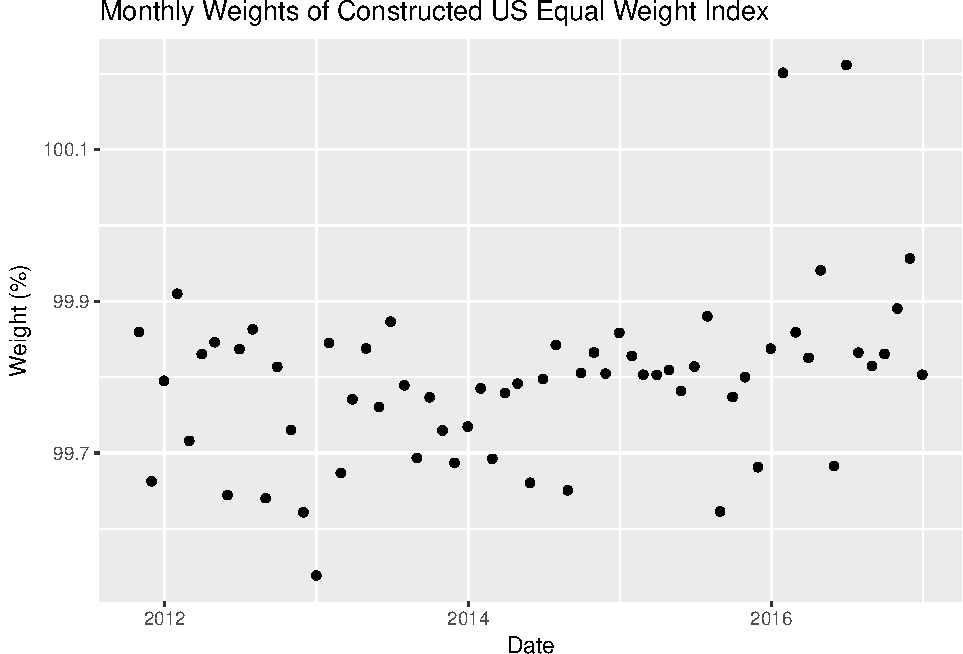
\includegraphics{thesis_files/figure-latex/unnamed-chunk-22-1.pdf}
\caption{\label{fig:unnamed-chunk-22}Weights of the constructed US Equal
Weight Index by month\label{fig:plot1}}
\end{figure}
\newline

The monthly change in weights for the constructed Minimum Volatility
Index is shown below in Figure \ref{fig:plot2}. The weights of the
constructed index are very close to 100\%, but with no value exceeding
that. The minimum weight is 99.58\%, while the largest weight is
99.99\%. The mean weight is 99.76\%.
\begin{figure}[htbp]
\centering
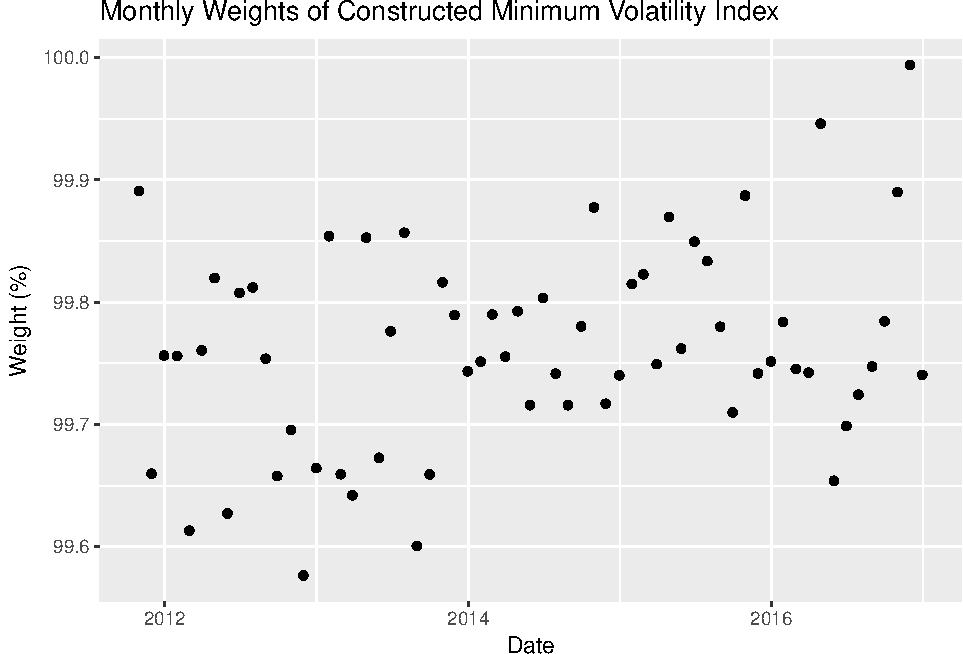
\includegraphics{thesis_files/figure-latex/unnamed-chunk-24-1.pdf}
\caption{\label{fig:unnamed-chunk-24}Weights of the constructed Minimum
Volatility Index by month\label{fig:plot2}}
\end{figure}
\subsection{Comparing ETF returns to Constructed Index
returns}\label{comparing-etf-returns-to-constructed-index-returns}

Given the weights were very close to 100\% for both constructed indices
on a monthly basis, an additional check was performed by comparing the
weighted returns of the constructed indices to the actual ETFs that
mirror them. The ETFs are traded in the stock market, so daily price
information on each was widely available. Thus, this provided a way to
check how the constructed weighted returns compared to the ETF returns
for both the constructed US Equal Weight Index and Minimum Volatility
Index. Correlations were calculated between the performance of the
constructed index and its ETF, and plotted over time. As shown in Figure
\ref{fig:plot3}, the overall correlation between the constructed US
Equal Weight Index monthly returns and EUSA ETF monthly returns was
98.06\%. As shown in Figure \ref{fig:plot4}, the overall correlation
between the constructed Minimum Volatility Index monthly returns and
USMV ETF monthly returns is 99.07\%.
\begin{figure}[htbp]
\centering
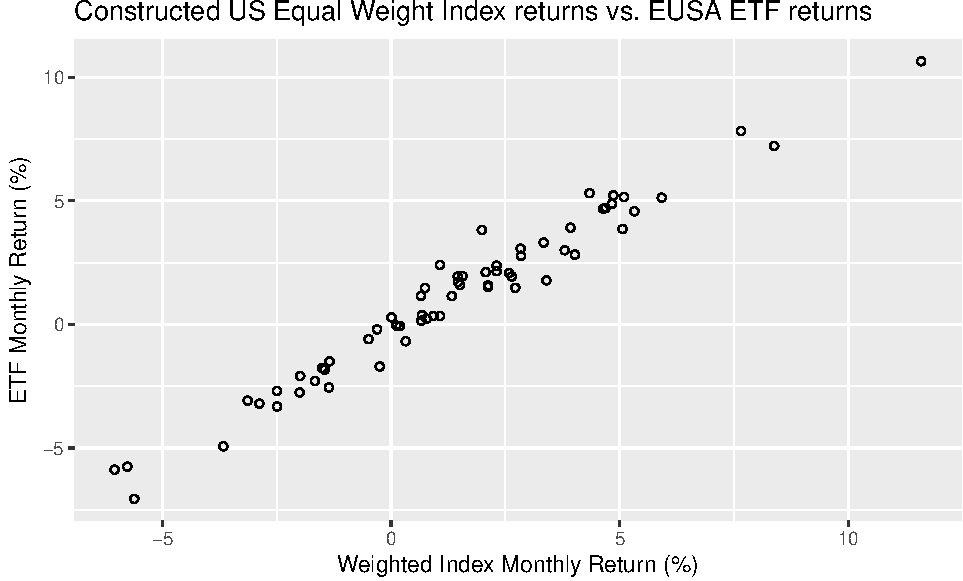
\includegraphics{thesis_files/figure-latex/unnamed-chunk-26-1.pdf}
\caption{\label{fig:unnamed-chunk-26}Correlations between constructed US
Equal Weight Index monthly returns and EUSA ETF monthly
returns\label{fig:plot3}}
\end{figure}
\begin{figure}[htbp]
\centering
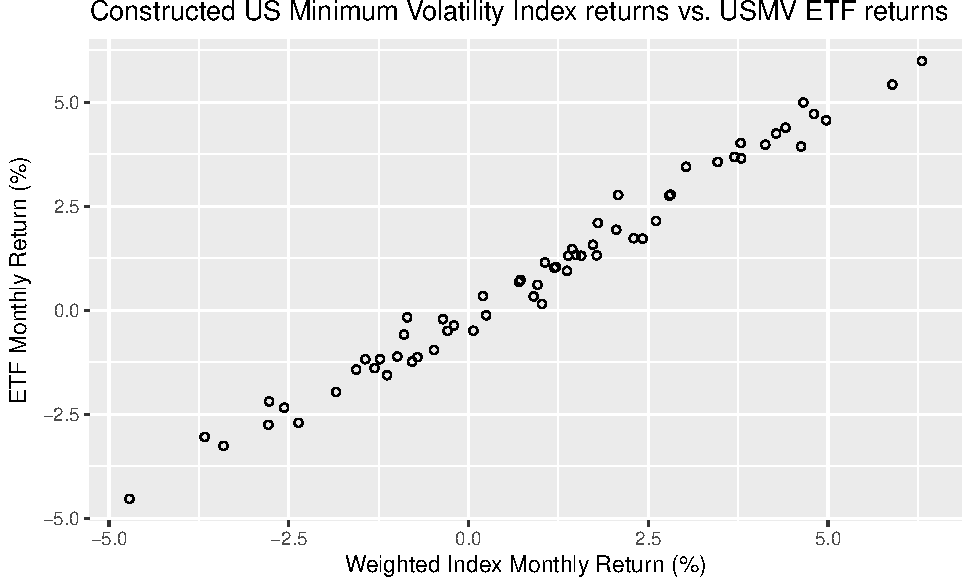
\includegraphics{thesis_files/figure-latex/unnamed-chunk-28-1.pdf}
\caption{\label{fig:unnamed-chunk-28}Correlations between constructed
Minimum Volatility Index monthly returns and USMV ETF monthly
returns\label{fig:plot4}}
\end{figure}
\chapter{Data Analysis}\label{data-analysis}

\section{Change in Largest Holdings Over
Time}\label{change-in-largest-holdings-over-time}

The top 5 largest holdings in the US Equal Weight Index by average
weight are Apple (AAPL), Exxon Mobil (XOM), Microsoft (MSFT), General
Electric (GE), and Johnson \& Johnson (JNJ). Each stock's average weight
is shown below in Table 4.1.
\begin{longtable}[t]{rlr}
\caption{\label{tab:unnamed-chunk-30}Average Weight of Top 5 Holdings in the US Equal Weight Index}\\
\toprule
Rank & Ticker & Average Weight (\%)\\
\midrule
1 & AAPL & 2.542271\\
2 & XOM & 1.946284\\
3 & MSFT & 1.315786\\
4 & GE & 1.157559\\
5 & JNJ & 1.135282\\
\bottomrule
\end{longtable}
The top 5 largest holdings in the Minimum Volatility Index by average
weight are Verizon (VZ), AT\&T (T), Automatic Data Processing (ADP),
Johnson \& Johnson (JNJ), and McDonald's (MCD). Each stock's average
weight is shown below in Table 4.2.
\begin{longtable}[t]{rlr}
\caption{\label{tab:unnamed-chunk-32}Average Weight of Top 5 Holdings in the Minimum Volatility Index}\\
\toprule
Rank & Ticker & Average Weight (\%)\\
\midrule
1 & VZ & 1.508046\\
2 & T & 1.493976\\
3 & ADP & 1.479657\\
4 & JNJ & 1.470513\\
5 & MCD & 1.458286\\
\bottomrule
\end{longtable}
The 5 largest holdings in the US Equal Weight index are AAPL, XOM, MSFT,
GE, and JNJ. As shown in Figure \ref{fig:plot5}, the weights of the 5
companies start off very high, each comprising a few percent of the
overall index, then suddenly all drop significantly to a fraction of a
percent after 2015-08-31. After verifying this with iShares and MSCI, it
was discovered that this due to change in the weighting
mechanism.\newline
\begin{figure}[htbp]
\centering
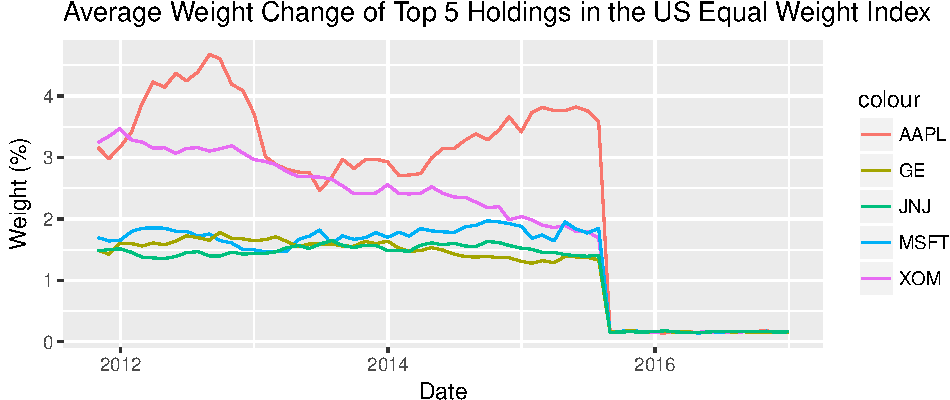
\includegraphics{thesis_files/figure-latex/unnamed-chunk-34-1.pdf}
\caption{\label{fig:unnamed-chunk-34}Change in weight for the top 5 holdings
in the US Equal Weight index over time\label{fig:plot5}}
\end{figure}
\newline
The 5 largest holdings of the Minimum Volatility index are VZ, T, ADP,
JNJ, and MCD. As shown in Figure \ref{fig:plot6}, since the index's
inception these stocks have generally oscillated between a weight of
1.3\% and 1.7\% of the overall portfolio, with the exception of Verizon
which reached around 2\% in 2014.
\begin{figure}[htbp]
\centering
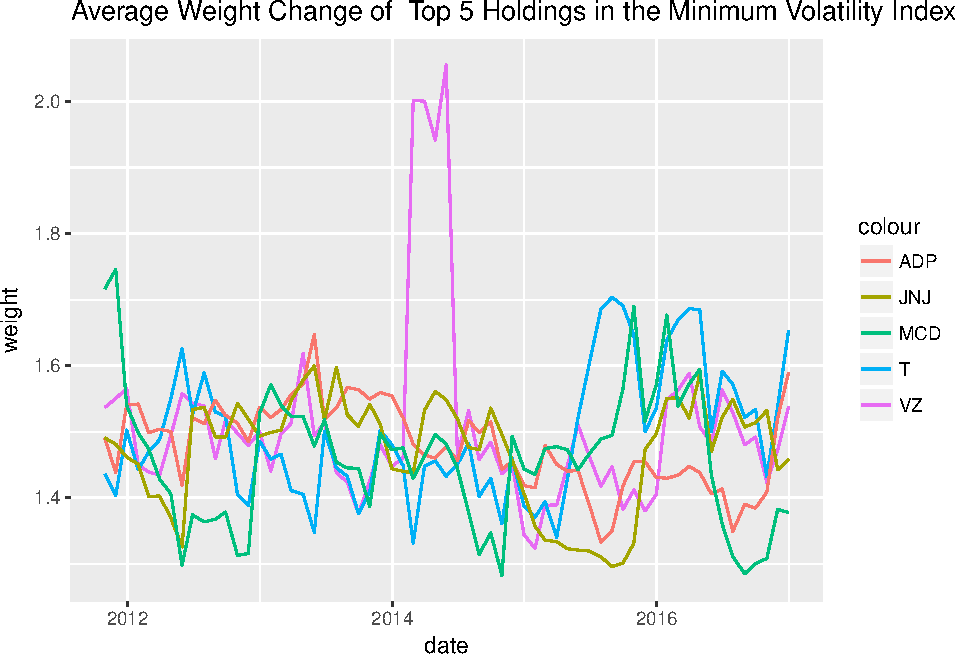
\includegraphics{thesis_files/figure-latex/unnamed-chunk-36-1.pdf}
\caption{\label{fig:unnamed-chunk-36}Change in weight for the top 5 holdings
in the Minimum Volatility index over time\label{fig:plot6}}
\end{figure}
\clearpage

\section{Change in Sector Weights Over
Time}\label{change-in-sector-weights-over-time}

Sector weights were calculated over time for both the US Equal Weight
and the Minimum Volatility Index by dividing the number of holdings for
each industry by the total number of holdings in the portfolio. This was
done to get a sense of what industries may be inherently more
``low-risk'' or ``high-risk.'' Moreover, this could help verify the
accuracy of the data, as each sector weighting in the Minimum Volatility
index should be within 5\% of each sector weighting in the US Equal
Weight Index, as specified by the Barra Open Optimizer (MSCI, 2013).

Shown below in Figure \ref{fig:sector1} are the sector weights over time
for energy stocks in both indices. The weighting of energy stocks in the
US Equal Weight Index is consistently greater than the weighting of
energy stocks in the Minimum Volatility Index. This could imply that by
nature, energy stocks are more volatile than stocks in other industries.
\begin{figure}[htbp]
\centering
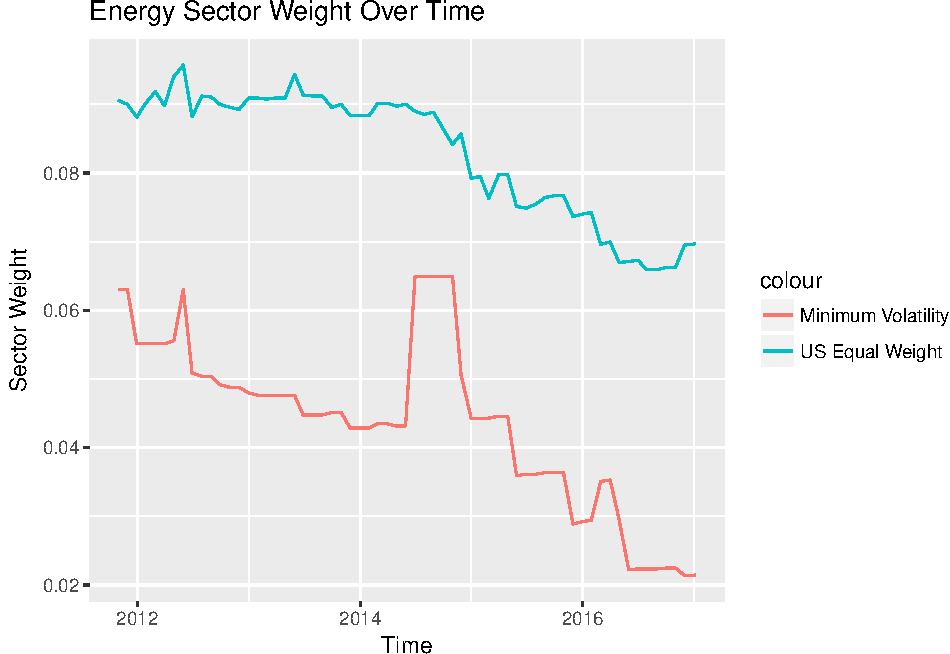
\includegraphics{thesis_files/figure-latex/unnamed-chunk-38-1.pdf}
\caption{\label{fig:unnamed-chunk-38}Weight of energy stocks by index over
time\label{fig:sector1}}
\end{figure}
\clearpage
Shown below in Figure \ref{fig:sector2} are the sector weights over time
for financial stocks in both indices. The weighting of financial stocks
in the US Equal Weight Index is fairly consistent, until a significant
drop towards the latter half of 2016. This timing coincides with the
Federal Reserve's decision to hike rates for just the second time in a
decade, amid positive economic signs (Cox, 2016). In the Minimum
Volatility Index, the weighting of financials fluctuate quite a bit, and
experience a similar drop in weight at that same point in time.
\begin{figure}[htbp]
\centering
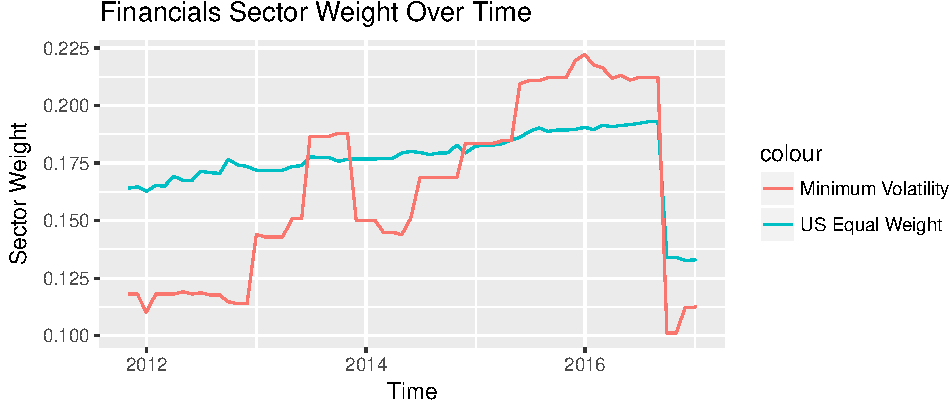
\includegraphics{thesis_files/figure-latex/unnamed-chunk-39-1.pdf}
\caption{\label{fig:unnamed-chunk-39}Weight of financial stocks by index
over time\label{fig:sector2}}
\end{figure}
\newline
Shown below in Figure \ref{fig:sector3} are the sector weights over time
for consumer staple stocks in both indices. The weighting of consumer
staples in the US Equal Weight Index is consistently lower than the
weighting of consumer staples in the Minimum Volatility Index. This
could imply that consumer staple stocks are less volatile than stocks in
other industries.
\begin{figure}[htbp]
\centering
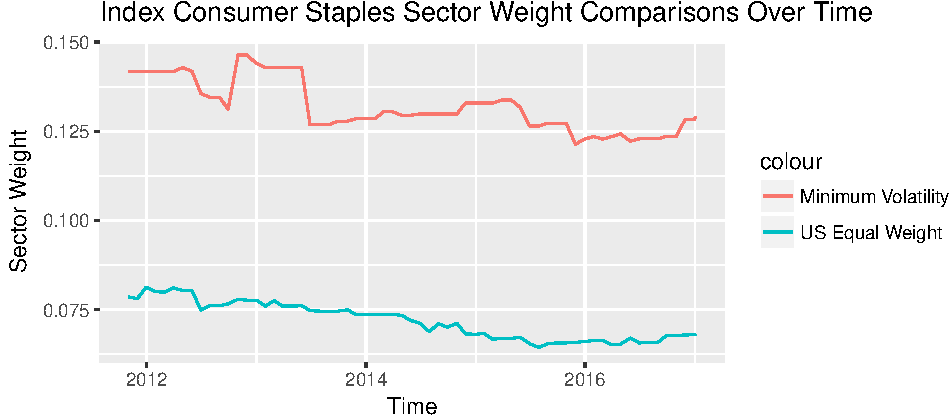
\includegraphics{thesis_files/figure-latex/unnamed-chunk-40-1.pdf}
\caption{\label{fig:unnamed-chunk-40}Weight of consumer staple stocks by
index over time\label{fig:sector3}}
\end{figure}
\clearpage
Shown below in Figure \ref{fig:sector4} are the sector weights over time
for consumer discretionary stocks in both indices. The weight of
consumer discretionary stocks is consistently greater in the US Equal
Weight Index than in the Minimum Volatility Index. This could imply that
consumer staple stocks are more volatile than stocks in other
industries.
\begin{figure}[htbp]
\centering
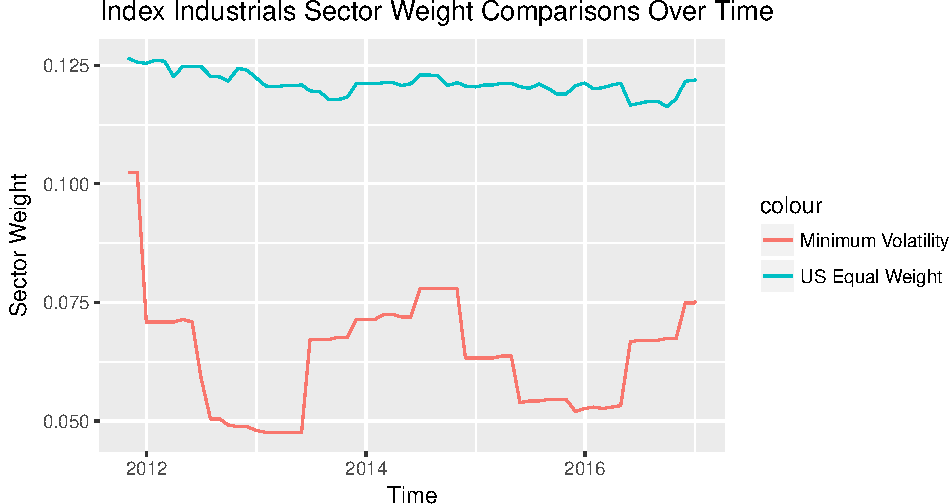
\includegraphics{thesis_files/figure-latex/unnamed-chunk-42-1.pdf}
\caption{\label{fig:unnamed-chunk-42}Weight of consumer discretionary stocks
by index over time\label{fig:sector4}}
\end{figure}
\newline
Shown below in Figure \ref{fig:sector5} are the sector weights over time
for healthcare stocks in both indices. The weight of healthcare stocks
is consistently higher over time in the Minimum Volatility Index than in
the US Equal Weight Index. This could imply that consumer staple stocks
are less volatile than stocks in other industries.
\begin{figure}[htbp]
\centering
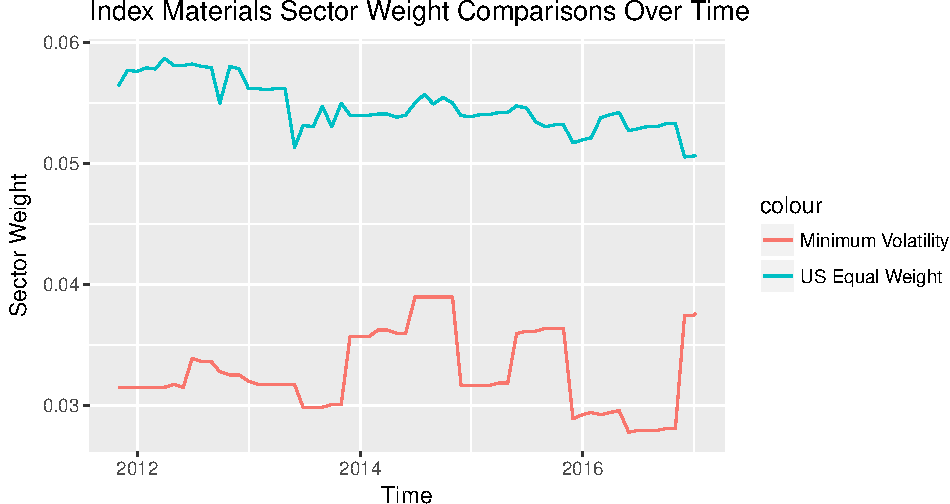
\includegraphics{thesis_files/figure-latex/unnamed-chunk-44-1.pdf}
\caption{\label{fig:unnamed-chunk-44}Weight of healthcare stocks by index
over time\label{fig:sector5}}
\end{figure}
\clearpage
Shown below in Figure \ref{fig:sector6} are the sector weights over time
for industrial stocks in both indices. The weight of industrials is
consistently higher over time in the US Equal Weight Index than in the
Minimum Volatility Index. This could imply that industrial stocks are
more volatile than stocks in other industries.
\begin{figure}[htbp]
\centering
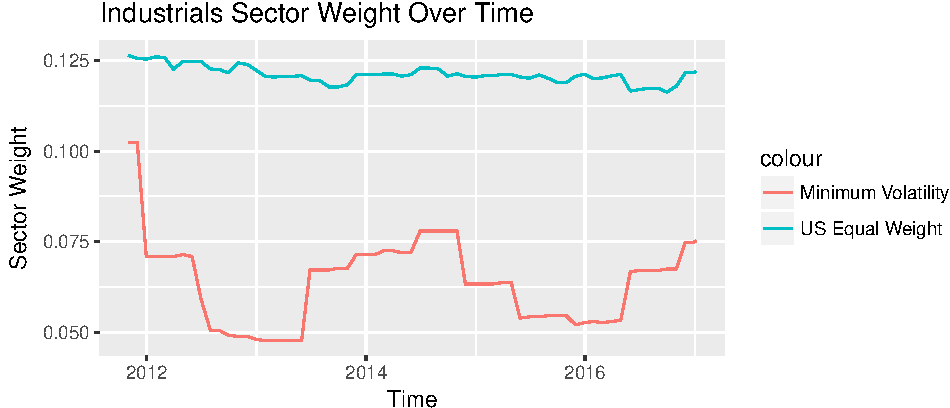
\includegraphics{thesis_files/figure-latex/unnamed-chunk-46-1.pdf}
\caption{\label{fig:unnamed-chunk-46}Weight of industrials stocks by index
over time\label{fig:sector6}}
\end{figure}
\newline
Shown below in Figure \ref{fig:sector7} are the sector weights over time
for information technology stocks in both indices. The weight of
information technology stocks between 2012 and 2013 was significantly
greater in the Minimum Volatility Index than in the US Equal Weight
Index. However, since 2014, the weights of IT in both indices have
converged, implying the industry may have become more volatile over the
last few years.
\begin{figure}[htbp]
\centering
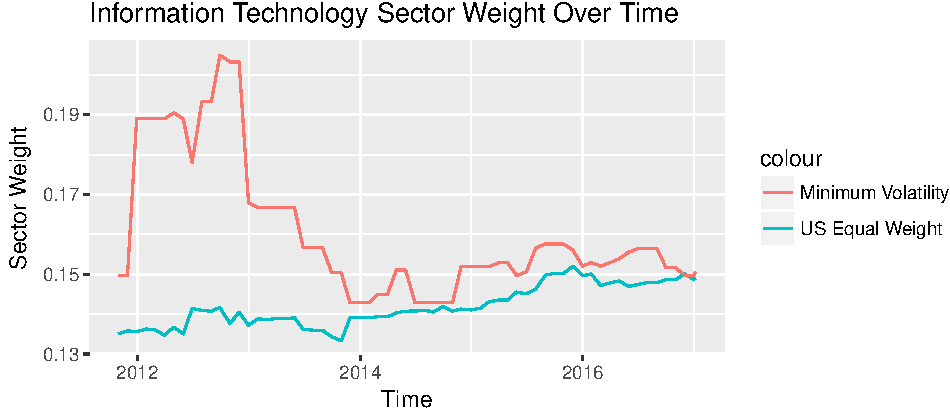
\includegraphics{thesis_files/figure-latex/unnamed-chunk-48-1.pdf}
\caption{\label{fig:unnamed-chunk-48}Weight of information technology stocks
by index over time\label{fig:sector7}}
\end{figure}
\clearpage
Shown below in Figure \ref{fig:sector8} are the sector weights over time
for materials stocks in both indices. The weight of materials is
consistently higher over time in the US Equal Weight Index than in the
Minimum Volatility Index. This could imply that materials companies may
be more volatile than companies in other sectors.
\begin{figure}[htbp]
\centering
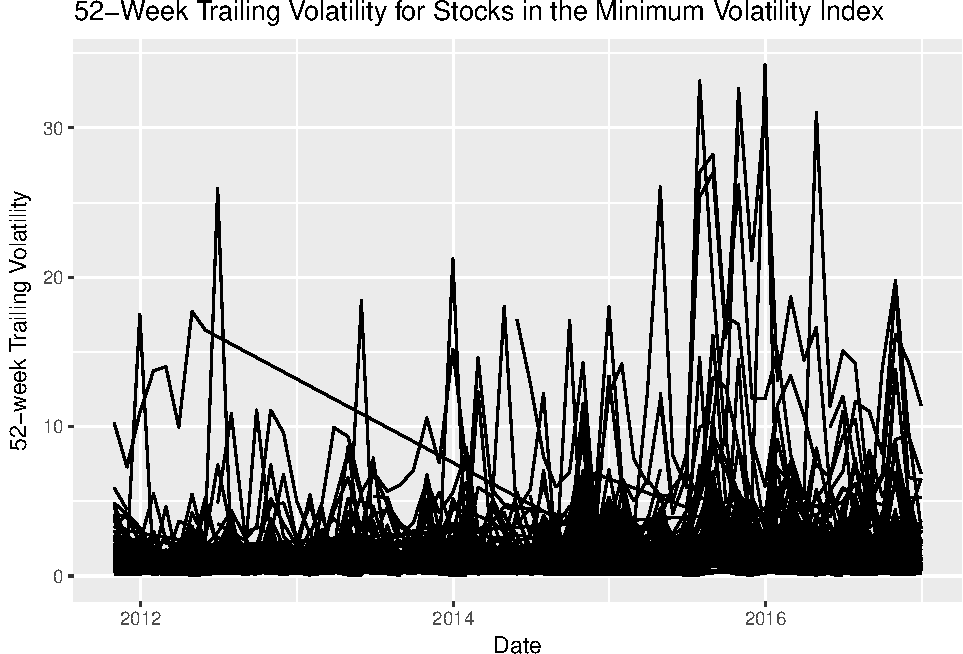
\includegraphics{thesis_files/figure-latex/unnamed-chunk-50-1.pdf}
\caption{\label{fig:unnamed-chunk-50}Weight of materials stocks by index
over time\label{fig:sector8}}
\end{figure}
\newline
Shown below in Figure \ref{fig:sector9} are the sector weights over time
for utilities stocks in both indices. The weight of utilities stocks is
higher over time in the Minimum Volatility Index than in the US Equal
Weight Index. This could imply that the utilities sector may not be as
volatile as other sectors.
\begin{figure}[htbp]
\centering
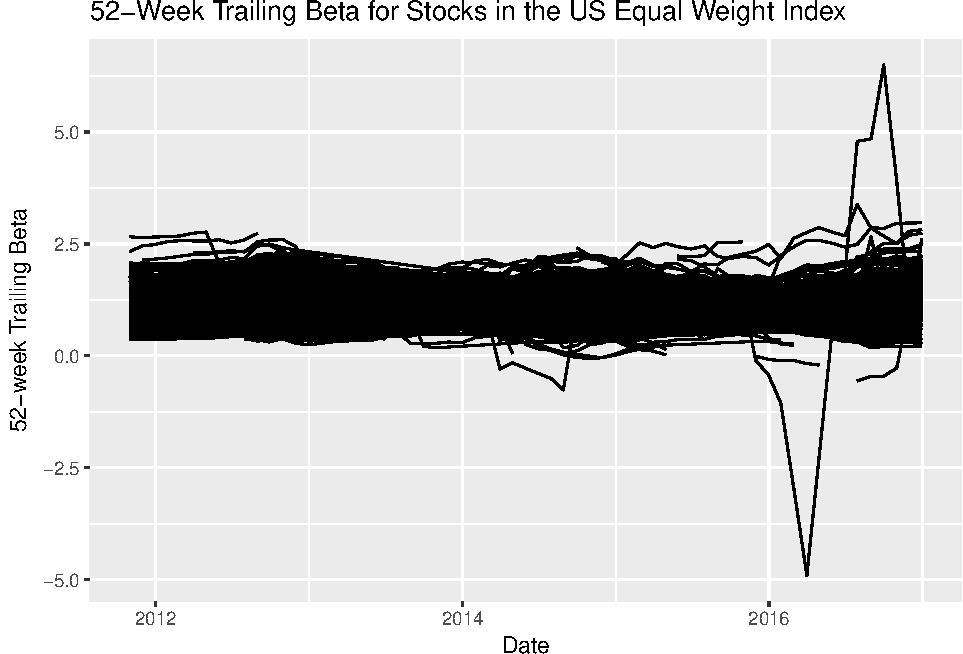
\includegraphics{thesis_files/figure-latex/unnamed-chunk-52-1.pdf}
\caption{\label{fig:unnamed-chunk-52}Weight of utilities stocks by index
over time\label{fig:sector9}}
\end{figure}
\clearpage
Shown below in Figure \ref{fig:sector10} are the sector weights over
time for telecommunications stocks in both indices. The weight of
telecommunications stocks is higher over time in the Minimum Volatility
Index than in the US Equal Weight Index. However, over time the weight
of telecommunications has consistently decreased, which would imply the
industry has gotten more volatile over the past few years.
\begin{figure}[htbp]
\centering
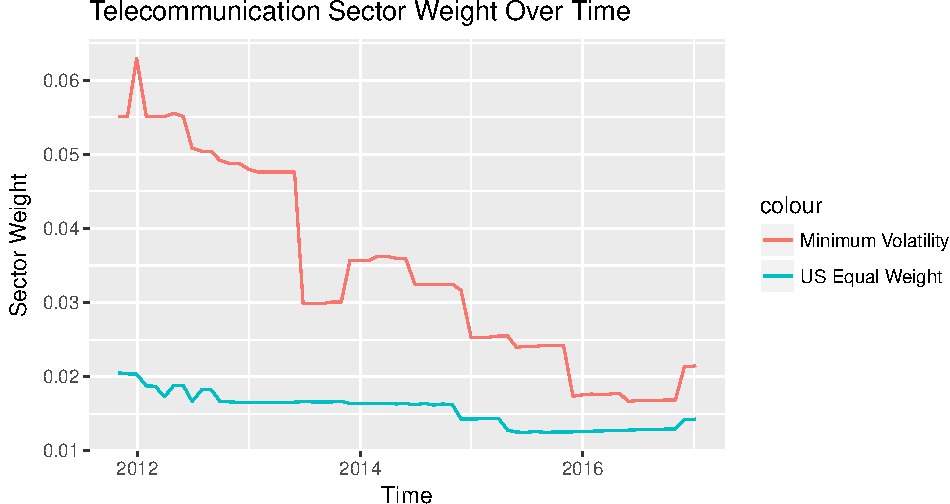
\includegraphics{thesis_files/figure-latex/unnamed-chunk-54-1.pdf}
\caption{\label{fig:unnamed-chunk-54}Weight of telecommunications stocks by
index over time\label{fig:sector10}}
\end{figure}
\clearpage 

\section{Trailing Volatility}\label{trailing-volatility}

Data was collected from 10/31/2010 to 12/30/2016, from Wharton Research
Data Services (WRDS) for the 908 historical constituents of the USA
Equal Weight (EUSA) ETF, of which the Minimum Volatility Index is
derived (Wharton Research Data Services, 2017). Each stock's 252-day
(annual) trailing volatility was calculated, and a month end spaghetti
plot was produced for stocks in the Minimum Volatility Index, and the
remainder of the stock comprising the US Equal Weight Index, to get a
relative sense of each group's volatility attributes. The stocks
comprising the Minimum Volatility Index generally had a lower volatility
than those in the US Equal Weight Index. Shown below in Figure
\ref{fig:vol1} are the 52-week trailing volatilities for stocks in the
US Equal Weight Index ranged from 0.00492 to 87.37030, with a mean value
of 1.44738.
\begin{verbatim}
    Min.  1st Qu.   Median     Mean  3rd Qu.     Max. 
 0.00492  0.50030  0.87466  1.44738  1.56562 87.37030 
\end{verbatim}
\begin{figure}[htbp]
\centering
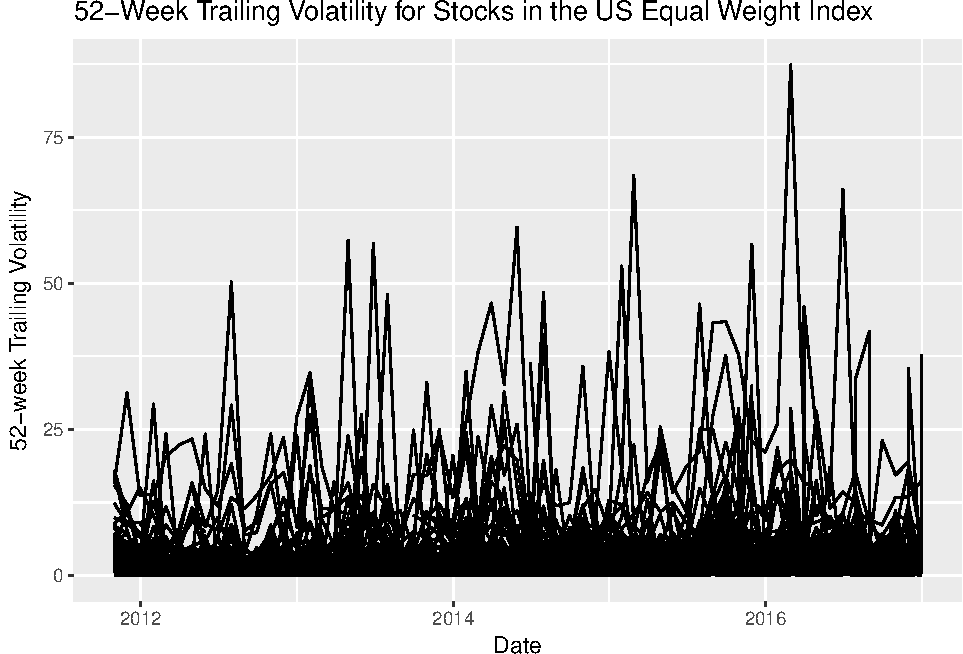
\includegraphics{thesis_files/figure-latex/unnamed-chunk-56-1.pdf}
\caption{\label{fig:unnamed-chunk-56}52-week trailing volatility for stocks
in the US Equal Weight Index\label{fig:vol1}}
\end{figure}
\clearpage  Shown below in Figure \ref{fig:vol2} are the 52-week
trailing volatilities for stocks in the Minimum Volatility Index ranged
from 0.03085 to 34.20974, with a mean value of 1.40784.
\begin{verbatim}
    Min.  1st Qu.   Median     Mean  3rd Qu.     Max. 
 0.03085  0.54767  0.91226  1.40784  1.51399 34.20974 
\end{verbatim}
\begin{figure}[htbp]
\centering
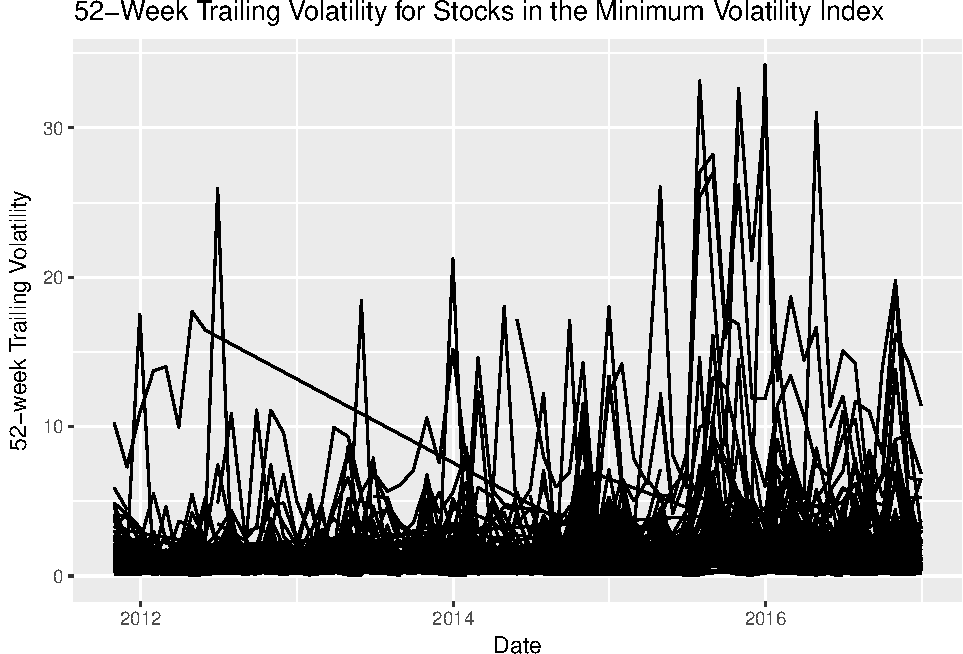
\includegraphics{thesis_files/figure-latex/unnamed-chunk-58-1.pdf}
\caption{\label{fig:unnamed-chunk-58}52-week trailing volatility for stocks
in the Minimum Volatility Index\label{fig:vol2}}
\end{figure}
\clearpage 

\section{Trailing Beta}\label{trailing-beta}

Data was collected from 10/31/2010 to 12/30/2016, from Wharton Research
Data Services (WRDS) for the 908 historical constituents of the USA
Equal Weight (EUSA) ETF, of which the Minimum Volatility Index is
derived (Wharton Research Data Services, 2017). Each stock's 252-day
(annual) trailing beta was calculated, and a month end spaghetti plot
was produced for stocks in the Minimum Volatility Index, and the
remainder of the stock comprising the US Equal Weight Index, to get a
relative sense of each group's volatility attributes. Generally, the
stocks comprising the Minimum Volatility Index had a lower beta than
those in the US Equal Weight Index. Shown below in Figure
\ref{fig:vol3}, the 52-week trailing beta for stocks in the US Equal
Weight Index ranged from -4.9037 to 6.4952, with a mean value of 1.1505.
\begin{verbatim}
   Min. 1st Qu.  Median    Mean 3rd Qu.    Max. 
-4.9037  0.9316  1.1250  1.1505  1.3512  6.4952 
\end{verbatim}
\begin{figure}[htbp]
\centering
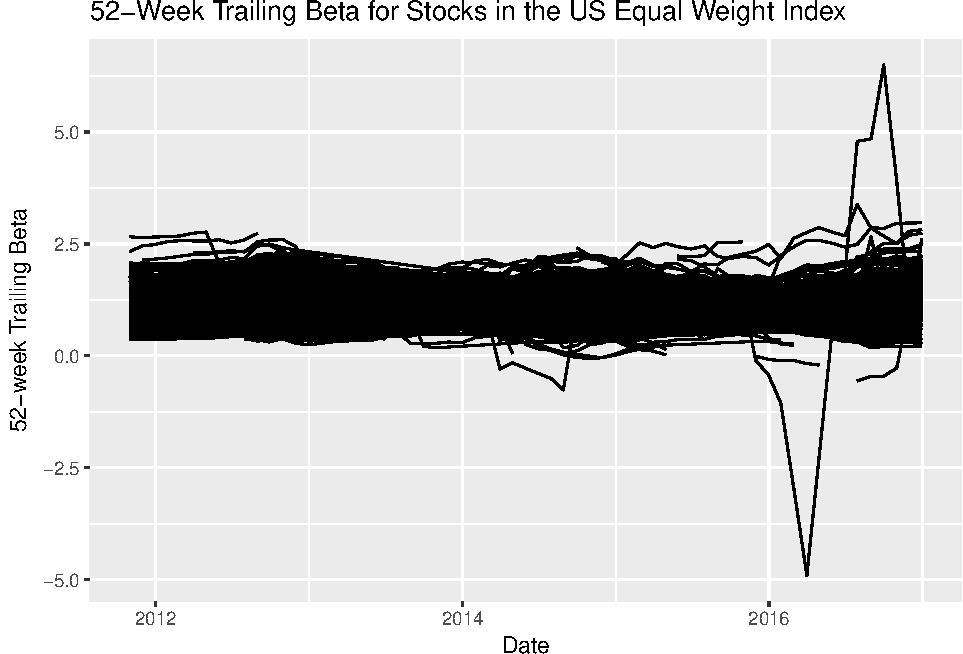
\includegraphics{thesis_files/figure-latex/unnamed-chunk-60-1.pdf}
\caption{\label{fig:unnamed-chunk-60}52-week trailing beta for stocks in the
US Equal Weight Index\label{fig:vol3}}
\end{figure}
\clearpage  Shown below in Figure \ref{fig:vol4}, the 52-week trailing
beta for stocks in the Minimum Volatility Index ranged from -0.2473 to
3.2021, with a mean value of 0.7856.
\begin{verbatim}
   Min. 1st Qu.  Median    Mean 3rd Qu.    Max. 
-0.2473  0.6319  0.7912  0.7856  0.9330  3.2021 
\end{verbatim}
\begin{figure}[htbp]
\centering
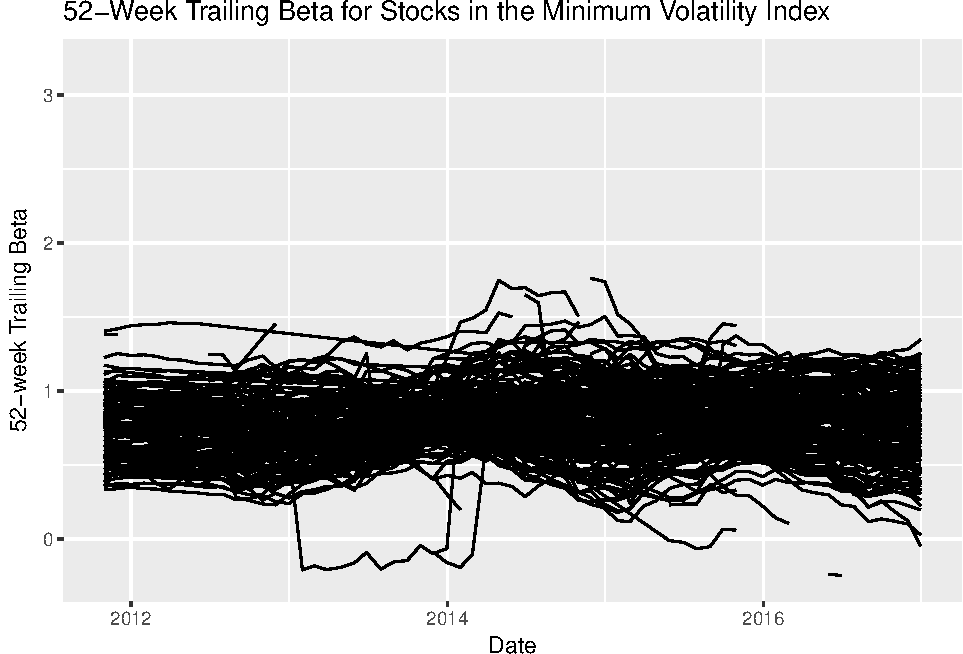
\includegraphics{thesis_files/figure-latex/unnamed-chunk-62-1.pdf}
\caption{\label{fig:unnamed-chunk-62}52-week trailing beta for stocks in the
Minimum Volatility Index\label{fig:vol4}}
\end{figure}
\chapter{Logistic Regression Model}\label{logistic-regression-model}

Once the final data set was created and cleaned, with a number of
response variables including trailing beta, trailing volatility, price
to book ratio, and the whether or not a stock was in the Minimum
Volatility index or not (1 if in, 0 if not in). Given the nature of the
data, a logistic regression was run. Looking at all of the historical
data and stock various characteristics, this modeled the log odds of a
stock being in the minimum volatility index as a combination of the
linear predictors mentioned. Since the index is rebalanced twice a year,
it makes sense to look at a model including the data for both of these
months.

\section{Data Cleaning}\label{data-cleaning-1}

\subsection{Removing Class Bias}\label{removing-class-bias}

Ideally, the proportion of stocks in and out of the Minimum Volatility
index should approximately be the same. However, after checking this, it
is clear that this is not the case, as there were 4182 observations for
stocks not in the index, and just 1385 observations for stocks in the
index. Since just around 25\% of the data was from stocks that are
currently in the index, there is class bias. As a result, observations
were sampled in equal proportions to get a better model.

\subsection{Creating Development and Test
Samples}\label{creating-development-and-test-samples}

One way to address the problem of class bias is to draw the 0's and 1's
for the development sample in equal proportions for a majority of the
observations. In doing so, the remaining data will not included for the
model, but will be used as the validation sample to evaluate and test
the model. Class bias was removed, as the sample is now evenly weighted,
with each outcome being represented by 969 observations. The remainder
of the data was placed in the validation sample.

\section{Logistic Regression Model}\label{logistic-regression-model-1}
\begin{verbatim}

Call:
glm(formula = index_now ~ volatility + beta + price_to_book + 
    index_before, family = binomial(link = "logit"), data = trainingData)

Deviance Residuals: 
    Min       1Q   Median       3Q      Max  
-3.4421  -0.3205   0.0156   0.2131   3.3425  

Coefficients:
                Estimate Std. Error z value Pr(>|z|)    
(Intercept)    1.858e+00  3.623e-01   5.128 2.93e-07 ***
volatility    -3.976e-02  4.072e-02  -0.977    0.329    
beta          -4.193e+00  3.933e-01 -10.661  < 2e-16 ***
price_to_book  5.059e-05  1.775e-02   0.003    0.998    
index_before1  5.432e+00  2.382e-01  22.802  < 2e-16 ***
---
Signif. codes:  0 '***' 0.001 '**' 0.01 '*' 0.05 '.' 0.1 ' ' 1

(Dispersion parameter for binomial family taken to be 1)

    Null deviance: 2686.64  on 1937  degrees of freedom
Residual deviance:  745.23  on 1933  degrees of freedom
AIC: 755.23

Number of Fisher Scoring iterations: 6
\end{verbatim}
To calculate the log odds of a stock being an index constituent:
\begin{figure}
$$ logit(p) = log(odds) = 1.858 - 0.03976 \times Volatlity - 4.193 \times Beta + 0.00005059 \times \frac{price}{book} + 5.432 \times index $$
\caption{Log Odds Equation}
\end{figure}
\hfill\break
To calculate the odds of a stock being an index constituent:
\begin{figure}
$$ odds = e ^ {1.858 - 0.03976 \times Volatlity - 4.193 \times Beta + 0.00005059 \times \frac{price}{book} + 5.432 \times index} $$
\caption{Odds Equation}
\end{figure}
\hfill\break
\hfill\break
\hfill\break
To calculate the probability of a stock being an index constituent:
\begin{figure}
$$ p = \frac {odds}{1 + odds} = \frac{e ^ {1.858 - 0.03976 \times Volatlity - 4.193 \times Beta + 0.00005059 \times \frac{price}{book} + 5.432 \times index}} {1 + e ^ {1.858 - 0.03976 \times Volatlity - 4.193 \times Beta + 0.00005059 \times \frac{price}{book} + 5.432 \times index}} $$
\caption{Probability Equation}
\end{figure}
\subsection{Coefficient
Interpretation}\label{coefficient-interpretation}

The coefficients can be interpreted as: \hfill\break
- Volatility: For a one unit increase in volatility, the log odds of a
stock being an index constituent change by -0.3976 \hfill\break
- Beta: For a one unit increase in beta, the log odds of a stock being
an index constituent change by -4.193 \hfill\break
- Price to Book: For a one unit change in price to book ratio, the log
odds of a stock being an index constituent increase by 0.00005059
\hfill\break
- Index before: For a one unit change in previous index membership, the
log odds of a stock being an index constituent increase by 5.432
\hfill\break

\section{Diagnostic Testing}\label{diagnostic-testing}

To test the quality of the model, several diagnostic tests were
performed: \hfill\break
\textbf{Variance Inflation Factors} \hfill\break
Variance inflation factors (VIF) are used in regressions to check for
multicollinearity, which occurs when one predictor variable can be
predicted from the others with a high degree of accuracy. An example of
this includes a person's height and weight, as these two variables are
very closely related. VIFs measure how much the variance of the
estimated regression coefficients in the model are inflated, compared to
a case when the predictor variables are linearly unrelated. The general
rule of thumb is that predictor variables with a VIF over 4 should be
further inspected, and variables with a VIF above 10 require correction.
As shown below, all the predictor variables in the model have VIFs well
below 4, indicating that multicollinearity is not a concern:
\begin{verbatim}
   volatility          beta price_to_book  index_before 
     1.018738      1.053972      1.020580      1.065880 
\end{verbatim}
\hfill\break
\textbf{Optimal Cutoff} \hfill\break
To get a sense of the model's predictive power, it is important to first
tune the optimal cutoff to improve the model by reducing
misclassification error. The default cutoff is often 0.5, but by tuning
the probability cutoff, the ability of the model to correctly predict
0's and 1's greatly improves. In this model, that cutoff was found to be
0.86.

\hfill\break
\textbf{Concordant and Discordant Pairs} \hfill\break
To calculate the number of concordant and discordant pairs, all the
possible pairs of 0's and 1's will be considered - that is, all the
pairs of observations for stocks not in the index, and stocks in the
index. In this data set, a total of 1,336,608 pairs were considered, and
the probability values for 0 and 1 were calculated for each. Thus,
considering each pair, which can be represented as (1,0), ranges for
cutoff values were determined based off of the probability of each
observed 0 and 1. Concordant pairs were noted when the cutoff value for
the 1 was higher than the cutoff value of the 0. Discordant pairs were
noted when this was not the case, and this was equivalent to the case
where the probability of the event was lower than the probability of a
non-event. These instances are contrary to the definition of the event
and non-event based off of the cutoff value calculated. In a perfect
model, 100\% of the pairs would be concordant. In this model, 96.8\% of
the pairs were concordant and 3.2\% of the pairs were discordant.

\hfill\break
\textbf{Misclassification Error} \hfill\break
Misclassification error measures the accuracy of the model by
determining what the percent mismatch is of the predicted outcomes
compared to the actual outcomes. By looking at the test data, this
quantifies how accurate the model was at predicting which stocks were in
the index and what stocks were not in the index, given their predictor
variable values. Better models will have lower misclassification errors.
In this logistic regression model, the misclassification error was
4.02\%.

\hfill\break
\textbf{Sensitivity and Specificity} \hfill\break
Sensitivity, also called the true positive rate, is the proportion of
stocks in the minimum volatility index that were correctly predicted by
the model. In the logistic regression model, the sensitivity was found
to be 86.29\%. Specificity, also called the true negative rate, is the
proportion of stocks not in the minimum volatility index that were
correctly predicted by the model, and can be calculated as 1 - False
Positive Rate. In the logistic regression model, the specificity was
found to be 98.19\%.

\hfill\break
\textbf{Confusion Matrix} \hfill\break
The confusion matrix is a table showing the total number of true
positives, true negatives, false positives, and false negatives from the
test data to evaluate the performance of a model. In this logistic
regression model, there were a total of 359 true positives, 3155 true
negatives, 58 false negatives, and 57 false positives. Shown below, the
columns are actuals outcomes, while the rows are predicted outcomes:
\begin{longtable}[t]{lrr}
\caption{\label{tab:unnamed-chunk-74}Regression Model Confusion Matrix}\\
\toprule
  & 0 & 1\\
\midrule
0 & 3155 & 57\\
1 & 58 & 359\\
\bottomrule
\end{longtable}
\hfill\break
\textbf{Receiver Operating Characteristics Curve} \hfill\break
The Receiver Operating Characteristics (ROC) Curve plots the true
positive rate (sensitivity) against the false positive rate
(1-specificity) for all different possible cutoffs. The area under the
curve is a measure of the accuracy of the model in distinguishing
between stocks in the index and stocks not in the index. A perfect model
would yield a ROC curve passing through the top left corner,
representing a sensitivity of 100\% and a specificity of 100\%, with an
area under the curve of 100\%. The area under the ROC curve for the
logistic regression model in this study is 96.77\%: \hfill\break
\begin{figure}

{\centering 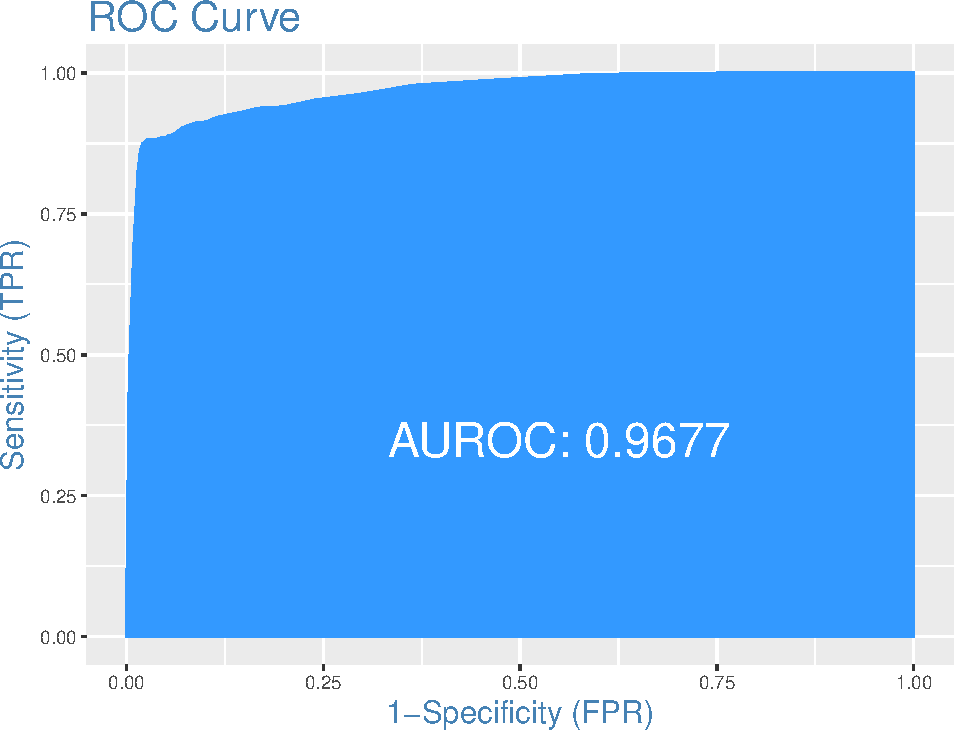
\includegraphics{thesis_files/figure-latex/unnamed-chunk-75-1} 

}

\caption{ROC Curve for Logistic Regression Model}\label{fig:unnamed-chunk-75}
\end{figure}
\hfill\break

\chapter{Conclusions and Future Work}\label{conclusions-and-future-work}

The logistic regression model was statistically resilient and had strong
predictive power. Based off of historical data, it was able to correctly
predict 86.29\% of stocks that were in the minimum volatility index, and
98.19\% of the stocks that were not members of the minimum volatility
index, using the optimal cut off. Overall, the logistic regression model
had a 96.77\% accuracy in distinguishing between stocks that were
members of the index, and stocks that were not members of the index. The
model can also be easily transformed to calculate the probability of a
stock being a member of the minimum volatility index based off of its
trailing beta, trailing volatility, price to book ratio, and prior index
membership.

\section{Understanding of
Relationships}\label{understanding-of-relationships}

The model can help build on previous understanding of what traits of a
stock are important in its membership in the minimum volatility index.
The relationship between trailing volatility and current membership in
the index was unsurprisingly negative; the larger a stock's volatility,
the less likely it is to be in the index. To be specific, the odds of
being in the index is 0.96 less with a one unit increase in a stock's
volatility. This makes sense, given the Barra Open Optimizer works to
create a minimum variance portfolio. The relationship between beta and
membership in the minimum volatility index was also negative; the larger
the magnitude of a stock's beta is, the less likely it is to be in the
index. To be specific, a one unit increase in a stock's beta makes it
0.015 times as likely to be in the index. This makes sense given that
beta is a measure of a stock's volatility as well. However, the
regression coefficient for beta was much stronger than the coefficient
for volatility, which at first glance appears puzzling, given that this
is a minimum volatility index. However, considering the units of each
variable can alleviate this concern; a one unit increase in volatility
in much less than a one unit increase in beta. For example, it would be
extremely very hard for a stock's beta to jump from 0.7 to 1.7 over a
short period of time, and would represent a massive change in a stock,
even though it is just one unit. This can help explain this coefficient
discrepancy, but it is important to note that both volatility and beta
are negatively related to index membership.

The relationship between price to book ratio and current membership in
the minimum volatility index was nonexistent in this model. In fact,
with a one unit increase in price to book ratio for a stock did not
affect a stock's odds of being a member of the index. This is an
interesting finding, in that it might imply a stock's value is unrelated
to its volatility, especially in relation to the importance of
profitability in defensive equity strategies (Novy-Marx, 2014). The
relationship between prior index membership and current membership in
the minimum volatility index was by far the most powerful. A stock was
over 228 times more likely to a member of the index if it was a member
six months ago. This is logical, considering a vast majority of the
stocks in the index remain. There are approximately 180 stocks in the
index, and during each rebalance only around 14 are removed (BlackRock,
2017).

\section{Sector-Specific Risk}\label{sector-specific-risk}

Some sectors were overweight or underweight in the minimum volatility
Index, which would imply something about sector-specific risk.
Macro-effects, like industry specific effects, have been shown to be
important in affecting risk and return of a portfolio (Baker et al.,
2014). Based off of the findings in this paper, energy, consumer
discretionary, industrials, and materials were shown to be consistently
underweight in the minimum volatility index when compared to the parent
index. This could mean these sectors are inherently more volatile than
other sectors. Moreover, consumer staples, healthcare, and utilities
were consistently overweight in the minimum volatility index when
compared to the parent index. This could imply that these sectors are
inherently less volatile than other sectors.

\section{Future Models}\label{future-models}

The logistic regression model took into account all of the data from the
months when rebalances took place. However, more specific models could
have been made to increase predictive power. Models could have been made
by using data by sector. As shown in the analysis, some sectors are more
volatile and risky than others, so using stocks without regard to sector
might lead to a less accurate model. Sector could also have been used as
a categorical predictor variable.

Seeing how significant of a predictor variable previous index membership
was in the regression model, it could make sense to create two separate
models: one for stocks currently in the minimum volatility index, and
one for stocks that are not. This could also help for investment
applications, as there will be one model used for short-selling stocks,
and one for deciding which stocks to purchase. Finally, creating models
by month could be telling too. By combining the May and November
rebalancing data, the current model does not take into account specific
factors that might be unique to rebalancing that occurs in either
period.

\section{Investment Implications}\label{investment-implications}

Given the accuracy and predictive power of the logistic regression
model, there are many ways it could be applied and used an investment
opportunity. If the model can accurately forecast index membership in
advance of its rebalancing, investors could long stocks that are
predicted to be added to the index, and short the stocks that are
expected to be removed from the index. Given that approximately 20
stocks are added and 14 stocks are removed during each rebalancing
(BlackRock, 2017), it could make sense to purchase stock in the top 5
companies that are currently not in the minimum volatility index but
have a high probability of being added, and short-sell stocks that are
currently in the minimum volatility but have a low probability of
remaining. When the iShares MSCI Minimum Volatility ETF is rebalanced,
stocks that were added enjoyed an average 0.63\% increase in price the
day after the announcement, and stocks that were removed lost 0.57\% of
value after the announcement. Though the values are small by themselves,
on an annualized basis, an accurate model could lead to a very lucrative
investment strategy.

\backmatter

\chapter*{References}\label{references}
\addcontentsline{toc}{chapter}{References}

\markboth{References}{References}

\noindent

\setlength{\parindent}{-0.20in} \setlength{\leftskip}{0.20in}
\setlength{\parskip}{8pt}

\hypertarget{refs}{}
\hypertarget{ref-adrian2014}{}
Adrian, T., Etula, E., \& Muir, T. (2014). Financial intermediaries and
the cross-section of asset returns. \emph{The Journal of Finance},
\emph{69}(6), 2557--2596.

\hypertarget{ref-amadeo2017}{}
Amadeo, K. (2017, april). Stock market crash of 2008. \emph{The
Balance}. Retrieved from
\url{https://www.thebalance.com/stock-market-crash-of-2008-3305535}

\hypertarget{ref-ang2006}{}
Ang, A., Hodrick, R. J., Xing, Y., \& Zhang, X. (2006). The
cross-section of volatility and expected returns. \emph{The Journal of
Finance}, \emph{61}(1), 259--299.

\hypertarget{ref-ang2009}{}
Ang, A., Hodrick, R. J., Xing, Y., \& Zhang, X. (2009). High
idiosyncratic volatility and low returns: International and further us
evidence. \emph{Journal of Financial Economics}, \emph{91}(1), 1--23.

\hypertarget{ref-asness2016}{}
Asness, C. S., Frazzini, A., Gormsen, N. J., \& Pedersen, L. H. (2016).
Betting against correlation: Testing theories of the low-risk effect.

\hypertarget{ref-baker2014}{}
Baker, M., Bradley, B., \& Taliaferro, R. (2014). The low-risk anomaly:
A decomposition into micro and macro effects. \emph{Financial Analysts
Journal}, \emph{70}(2), 43--58.

\hypertarget{ref-baker2011}{}
Baker, M., Bradley, B., \& Wurgler, J. (2011). Benchmarks as limits to
arbitrage: Understanding the low-volatility anomaly. \emph{Financial
Analysts Journal}, \emph{67}(1), 40--54.

\hypertarget{ref-beneish1996}{}
Beneish, M. D., \& Whaley, R. E. (1996). An anatomy of the ``s\&P
game'': The effects of changing the rules. \emph{The Journal of
Finance}, \emph{51}(5), 1909--1930.

\hypertarget{ref-berger2017}{}
Berger, R. (2017, May). Amazon's 49,000. \emph{Forbes}. Forbes Magazine.
Retrieved from
\url{https://www.forbes.com/sites/robertberger/2017/05/20/amazons-49000-return-a-test-for-value-investors/\#7b8efe2049cf)}

\hypertarget{ref-blackrock2017}{}
BlackRock. (2017, September). IShares edge msci min vol usa etf
\textbar{} usmv. Retrieved from
\url{https://www.ishares.com/us/products/239695/ishares-msci-usa-minimum-volatility-etf}

\hypertarget{ref-boyer2009}{}
Boyer, B., Mitton, T., \& Vorkink, K. (2009). Expected idiosyncratic
skewness. \emph{The Review of Financial Studies}, \emph{23}(1),
169--202.

\hypertarget{ref-brennan1989}{}
Brennan, M. J. (1989). Capital asset pricing model. In \emph{Finance}
(pp. 91--102). Springer.

\hypertarget{ref-chan1991}{}
Chan, L. K., Hamao, Y., \& Lakonishok, J. (1991). Fundamentals and stock
returns in japan. \emph{The Journal of Finance}, \emph{46}(5),
1739--1764.

\hypertarget{ref-chen2004}{}
Chen, H., Noronha, G., \& Singal, V. (2004). The price response to s\&P
500 index additions and deletions: Evidence of asymmetry and a new
explanation. \emph{The Journal of Finance}, \emph{59}(4), 1901--1930.

\hypertarget{ref-cox2016}{}
Cox, J. (2016, December). Fed raises rates for the second time in a
decade. Retrieved from
\url{https://www.cnbc.com/2016/12/14/fed-raises-rates-for-the-second-time-in-a-decade.html}

\hypertarget{ref-falkenstein2012}{}
Falkenstein, E. G. (2012). \emph{The missing risk premium: Why low
volatility investing works}. Eric Falkenstein.

\hypertarget{ref-fama1992}{}
Fama, E. F., \& French, K. R. (1992). The cross-section of expected
stock returns. \emph{The Journal of Finance}, \emph{47}(2), 427--465.

\hypertarget{ref-fischhoff1977}{}
Fischhoff, B., Slovic, P., \& Lichtenstein, S. (1977). Knowing with
certainty: The appropriateness of extreme confidence. \emph{Journal of
Experimental Psychology: Human Perception and Performance}, \emph{3}(4),
552.

\hypertarget{ref-fontinelle2009}{}
Fontinelle, E. (2009, October). ETF tracking errors: Protect your
returns. Retrieved from
\url{http://www.investopedia.com/articles/exchangetradedfunds/09/tracking-error-etf-funds.asp}

\hypertarget{ref-frazzini2014}{}
Frazzini, A., \& Pedersen, L. H. (2014). Betting against beta.
\emph{Journal of Financial Economics}, \emph{111}(1), 1--25.

\hypertarget{ref-goodwin1998}{}
Goodwin, T. H. (1998). The information ratio. \emph{Financial Analysts
Journal}, \emph{54}(4), 34--43.

\hypertarget{ref-graham1965}{}
Graham, B. (1965). \emph{The intelligent investor: A book of practical
counsel}. Prabhat Prakashan.

\hypertarget{ref-harris1986}{}
Harris, L., \& Gurel, E. (1986). Price and volume effects associated
with changes in the s\&P 500 list: New evidence for the existence of
price pressures. \emph{The Journal of Finance}, \emph{41}(4), 815--829.

\hypertarget{ref-haugen1975}{}
Haugen, R. A., \& Heins, J. A. (1975). Risk and the rate of return on
financial assets: Some old wine in new bottles. \emph{Journal of
Financial and Quantitative Analysis}, \emph{10}(5), 775--784.

\hypertarget{ref-hayes2017}{}
Hayes, A. (2017, October). Exchange-traded fund (etf). Retrieved from
\url{http://www.investopedia.com/terms/e/etf.asp}

\hypertarget{ref-history2010}{}
History. (2010). Stock market crash of 1929. \emph{History.com}. A\&E
Television Networks. Retrieved from
\url{http://www.history.com/topics/1929-stock-market-crash}

\hypertarget{ref-huij2016}{}
Huij, J., \& Kyosev, G. (2016). Price response to factor index additions
and deletions.

\hypertarget{ref-investopedia2015}{}
Investopedia. (2015, April). What are some common measures of risk used
in risk management? \emph{Investopedia}. Retrieved from
\url{http://www.investopedia.com/ask/answers/041415/what-are-some-common-measures-risk-used-risk-management.asp}

\hypertarget{ref-investopedia2017}{}
Investopedia. (2017, February). Two and twenty. \emph{Investopedia}.
Retrieved from
\url{http://www.investopedia.com/terms/t/two_and_twenty.asp}

\hypertarget{ref-jensen1972}{}
Jensen, M. C., Black, F., \& Scholes, M. S. (1972). The capital asset
pricing model: Some empirical tests.

\hypertarget{ref-karceski2002}{}
Karceski, J. (2002). Returns-chasing behavior, mutual funds, and beta's
death. \emph{Journal of Financial and Quantitative Analysis},
\emph{37}(4), 559--594.

\hypertarget{ref-macdonald2009}{}
MacDonald, L. (2009). How traders are front-running etfs. Retrieved from
\url{https://seekingalpha.com/article/165877-how-traders-are-front-running-etfs}

\hypertarget{ref-msci2013}{}
MSCI. (2013, September). Barra open optimizer. Retrieved from
\url{https://www.msci.com/documents/10199/242721/Barra_Optimizer.pdf/5acf4515-dbd8-4d0c-8acc-ca70b7b68f69}

\hypertarget{ref-mullins1982}{}
Mullins, D. W. (1982). Does the capital asset pricing model work.
\emph{Harvard Business Review}, \emph{60}(1), 105--113.

\hypertarget{ref-novy2014}{}
Novy-Marx, R. (2014). Understanding defensive equity.

\hypertarget{ref-ontario2017}{}
Ontario, S. C. (2017, May). Types of investment risk \textbar{}
understanding risk. Retrieved from
\url{https://www.getsmarteraboutmoney.ca/invest/investing-basics/understanding-risk/types-of-investment-risk/}

\hypertarget{ref-pettengill1995}{}
Pettengill, G. N., Sundaram, S., \& Mathur, I. (1995). The conditional
relation between beta and returns. \emph{Journal of Financial and
Quantitative Analysis}, \emph{30}(1), 101--116.

\hypertarget{ref-rstudio2017}{}
RStudio Team. (2015). \emph{RStudio: Integrated development environment
for r}. Boston, MA: RStudio, Inc. Retrieved from
\url{http://www.rstudio.com/}

\hypertarget{ref-sec2017}{}
SEC. (2017, January). Mutual funds and exchange-traded funds (etfs) -- a
guide for investors. Retrieved from
\url{https://www.sec.gov/reportspubs/investor-publications/investorpubsinwsmfhtm.html}

\hypertarget{ref-sensoy2009}{}
Sensoy, B. A. (2009). Performance evaluation and self-designated
benchmark indexes in the mutual fund industry. \emph{Journal of
Financial Economics}, \emph{92}(1), 25--39.

\hypertarget{ref-shleifer1986}{}
Shleifer, A. (1986). Do demand curves for stocks slope down? \emph{The
Journal of Finance}, \emph{41}(3), 579--590.

\hypertarget{ref-van2016}{}
Vliet, P. V., \& Koning, J. de. (2016). \emph{High returns from low
risk: A remarkable stock market paradox}. John Wiley \& Sons.

\hypertarget{ref-wrds2017}{}
Wharton Research Data Services. (2017, May). WRDS data. Retrieved from
\url{https://wrds-web.wharton.upenn.edu/wrds/}

\hypertarget{ref-wynne2016}{}
Wynne, B. (2016). Understanding the iShares msci usa minimum volatility
etf. Retrieved from
\url{https://seekingalpha.com/article/3964639-understanding-ishares-msci-usa-minimum-volatility-etf}


% Index?

\end{document}
